%  University of Houston PhD proposal
%
% on  PC
%\documentclass[12pt]{report}
% \usepackage{uhthesis}
% \usepackage[pctex32]{graphics}
% \usepackage[pctex32]{color}
%\usepackage{psfig}
\documentclass[12pt]{report}
\usepackage{uhthesis3}
\usepackage{epsfig}
\usepackage{epsf}

% LAD definitions
\def\vx{{\vec x}}
\def\vxdot{{\dot\vx}} \def\vxddot{{\ddot\vx}}
\def\tpose{^\top}
\def\ru{{\rm u}}
\def\vc{{\vec c}}
\def\vrho{{{\bf p}}}
\def\mat#1{{\bf#1}}
\def\vec#1{{\bf#1}}
\def\bold#1{\setbox0=\hbox{#1}
 \kern-.025em\copy0\kern-\wd0
 \kern.05em\copy0\kern-\wd0
 \kern-.025em\raise.0433em\box0}
\def\vsigma{{\bf \sigma}}
\def\vepsilon{{\bf \epsilon}}
\def\ssqueeze{\vspace{-0.5cm}}

\def\bsqueeze{\vspace*{-0.8cm}}
\def\bpsqueeze{\vspace*{-0.6cm}}
\def\asqueeze{\vspace{-0.5cm}}


\def\inv{^{-1}}
\def\vuhat{{\hat \vec u}}
\def\avtk{{t_{k}}}
\def\bvtk{{t_{k+1}}}
\def\vu{{\vec u}}
\def\vuhat{{\hat \vec u}}
\def\vq{{\vec q}}
\def\vqdot{{\dot\vq}}
\def\tpose{^\top}
\def\mat#1{{\bf#1}}
\def\extvec#1#2#3{{~^{#1}{\bf#2}_{#3}}}
\def\extvecrm#1#2#3{{~^{{\rm #1}}{\bf#2}_{#3}}}

\def\cavindex{{\cal V\cal I}}
\def\caawpoint{{\extvec{\Phi}{x}{j}}}
\def\caaipointrm{{\extvecrm{I}{x}{j}}}
\def\caaipoint{{\extvec{I}{x}{j}}}

\newcounter{lfigcounter}
\newenvironment{IonTab}{\begin{table}[htb]}{\end{table}}
\newenvironment{IonFig}{\setcounter{lfigcounter}{1}\begin{figure}}{\end{figure}}
\newenvironment{IonFigH}{\setcounter{lfigcounter}{1}\begin{figure}[h]}{\end{figure}}
\newenvironment{IonFigT}{\setcounter{lfigcounter}{1}\begin{figure}[t]}{\end{figure}}
\def\ionbox#1{\makebox[#1]{(\alph{lfigcounter})}\stepcounter{lfigcounter}}

%%%%%%%%%%%%%%%%%%%%%%%%%%%%%%%%%%%%%%%%%%%%%%%%%%%%%%%%%%%%%%


\usepackage{url}
\usepackage{float}
\usepackage{subfigure}
\usepackage{siunitx}
\usepackage{amsmath,amssymb}
\usepackage{lscape}
\usepackage{algpseudocode}
\usepackage{algorithm}
\usepackage{mathtools}
\usepackage[justification=centering]{caption}

 
\usepackage[%
%\ifpdf
 pdftex,
%\else
% dvipdf,
%\fi
% ps2pdf, % using ps2pdf vs pdftex
% colorlinks=true, % color the words instead of use a colored box
% urlcolor=blue, % \href{...}{...} external (URL)
% filecolor=blue, % \href{...} local file
% linkcolor=black, % \ref{...} and \pageref{...}
% citecolor=black, % \cite{}
pdfborder={0 0 0}, % for removing borders around links
plainpages=false,
% plainpages boolean true
% Forces page anchors to be named by the arabic form of the page number,
% rather than the formatted form.
breaklinks=true,
% breaklinks boolean false
% Allows link text to break across lines; since this cannot be accommodated in
% PDF, it is only set true by default if the pdftex driver is used. This makes
% links on multiple lines into different PDF links to the same target.
pagebackref=true,
% Adds ?backlink? text to the end of each item in the bibliography, as a list
% of section numbers. This can only work properly if there is a blank line
% after each \bibitem.
bookmarksnumbered=true,
% bookmarksnumbered boolean false
% If Acrobat bookmarks are requested, include section numbers.
bookmarksopen=true,
% bookmarksopen boolean false
% If Acrobat bookmarks are requested, show them with all the subtrees expanded.
pdftitle={},
pdfauthor={},
pdfsubject={},
pdfkeywords={},
pdfpagelabels=true,
pdfpagemode=UseOutlines % None, UseThumbs, UseOutlines, FullScreen
]{hyperref}


\algnewcommand{\LineComment}[1]{\State \(\triangleright\) #1}
\renewcommand*{\arraystretch}{1.2}

\DeclarePairedDelimiter\ceil{\lceil}{\rceil}
\DeclarePairedDelimiter\floor{\lfloor}{\rfloor}
%\input{algorithms}
%
%
%
% on UNIX LATEX and Windows PCTEX32
%\documentstyle[12pt,uhthesis1,psfig]{report}
%\usepackage{epsfig}
%\input{algorithms}
%\input{psfig}
%\input{dnmmath}
%\input{ion-math}

%begin add from saso paper, check if ok for UH template

\newcommand{\bi}{\begin{itemize}}
\newcommand{\ei}{\end{itemize}}
\newcommand{\be}{\begin{equation}}
\newcommand{\ee}{\end{equation}}
\newcommand{\bd}{\begin{displaymath}}
\newcommand{\ed}{\end{displaymath}}
\newcommand{\myvec}[1] % Vektor
   {\mathbb{#1}}
%\newcommand{\mat}[1] % Matrix
%   {\mathsf{#1}}
%end add

\setcounter{secnumdepth}{4}
\begin{document}
% Bismillahirrahmanirrahim
%Bismilleh Arrahman Arrahim
%first title tentative
\title{\bf \large Automated Segmentation, Analysis and Classification of Zebrafish Vasculature }
% Runtime / Dynamic / On the fly
% Adaptation / Optimization /  Tuning
\author{Charu Hans}
%pre - defense date -> defense date then
\submitdate{May 2015} \degree{Doctor of Philosophy}{Dissertation}
\adviser{Shishir Shah, Chairman\\
Dept. of Computer Science }

\firstreader{Edgar Gabriel \\
Dept. of Computer Science}

\secondreader{Guoning Chen\\
Dept. of Computer Science}

\thirdreader{Fatima Merchant\\
Dept. of Engineering Technology, \\
College of Technology}

\fourthreader{Maria Bondesson\\
Dept. of Biology and Biochemistry}

\copyrightfalse \makecoverpages
\begin{acknowledgements}
%\input{acknowledgements.tex}
\end{acknowledgements}

\begin{abstract}
An important factor facilitating the application of zebrafish in biomedical research is high throughput screening of vertebrate animal models. Presently, the zebrafish has become a viable model for various research including vertebrate development, gene expression analysis, human diseases modeling, drug screening and toxicology analysis. Compared to other models, the zebrafish embryo is an attractive model due its fast development, small size, transparent embryos that develop outside the mother, and the availability of a large selection of mutant strains. However, the lack of tools for automated analysis of complex images is a huge bottleneck in utilizing the zebrafish to its full potential. 

Zebrafish have a closed circulatory system, and the mechanism of vessel formation are highly similar to those in humans. Being able to model the growth of blood vessel in the vasculature system of zebrafish is interesting for understanding both the circulatory system in humans, and for facilitating large scale screening of the influence of various chemicals on vascular development. Compared to other models, the zebrafish embryo is an attractive alternative for environmental risk assessment of chemicals since it offers the possibility to perform high throughput analysis in vivo. Intersegmental vessels (ISV) and caudal vein plexus (CVP) undergoes active development via angiogenesis. Hence, providing excellent models to study vasculature system.

Most of the current research based on ISV observe the presence or absence of ISVs or perturbation of ISV morphology but do not quantify growth dynamics. Moreover, these analysis are done manually hence it is tedious and expensive. All of these factors facilitate the need for automated image processing methods to quantitatively analyze the image dataset. In this work, we have focused on developing an image processing algorithm to automatically segment and quantify ISVs of zebrafish embryos that have been treated by various toxins. We tested the algorithm on images of zebrafish embryos obtained from screening compounds that may act as an ISV disruptor. The efficiency of segmentation approach is demonstrated by our experiments of the entire zebrafish vasculature recorded from the fluorescence microscope. The experiments also demonstrate that automated segmentation of ISV is comparable to that of manual segmentation. The quantified features are used to train a linear SVM classifier to identify morphological changes in a dataset consisting of ISV zebrafish embryo images. 

%We have also presented work for time-lapse confocal imaging of embryonic vasculature in the zebrafish using image analysis to monitor and quantify the effect of toxins on vascular development.

Recently, studies have indicated that zebrafish CVP also undergoes active development, hence providing an additional measure for studying vascular development. In this work, we have presented an approach to segment and detect abnormalities in the CVP region of zebrafish embryos due to exposure to toxins.  Morphological changes due to toxin exposure is modeled based on the proposed gradient weighted co-occurrence histogram of oriented gradients (gCo-HOG). These features are compared to more commonly used histogram of oriented gradients (HOG) features and Co-HOG features that utilizes spatial distribution of neighboring pixels to capture spatial structure. The features are used to train a linear SVM classifier to identify morphological changes in a dataset of region of CVP zebrafish embryo images.

\end{abstract}
\setlength{\parskip}{.1 in}

\makecontentspages

%uncomment the following for single space drafts
%\singlespace

% \pagenumbering{romans}{1}
% \beforepreface

%\pagestyle(empty}\times


%%%%%%%%%%%%%%%%%%%%%%%%%%%%%%%%%%%%%%%%%%%%%%%%%%%%%%%%%%%%%%%%%%%%



\chapterpages

%turn figures on and off
\newif \ifFIGS

%\FIGStrue

\FIGSfalse


%\tablelistfalse

%\listoftables

% to fix the page number
%\input{Sample_chapter.tex}
%\input{table.tex}
\chapter{Introduction}\label{chap:Intro}

\section{Motivation}

Zebrafish has recently emerged as an invaluable model for biomedical research. Enormous amounts of data is being generated from imaging zebrafish embryos. Manual image analysis is cumbersome and subjective, there by increasing the need for automated image analysis tools. Lack of automated image processing tools for zebrafish analysis is a huge bottleneck in realizing zebrafish application to its full potential.

\par
The growing utility of zebrafish as a model for biomedical research is attributed to its properties such as transparency, reproducibility, growth rate, and small size. The transparency of zebrafish embryo makes it a good model for direct observation of the development of organs and tissue. For this reason, zebrafish has been widely utilized to study neural developmental \cite{campbell2006}, and vasculature development \cite{fouquet1997}. It enables researchers to study different development stages of zebrafish to adulthood \cite{Kimmel95}. Transparent zebrafish promotes relatively easy modification of genetic expressions to mimic various diseases including Cancer \cite{Amatruda08}, Alzheimer \cite{Newman11}, and Parkinsons \cite{Boehmler09}. Neuronal structures and blood vessels can be directly observed, providing an opportunity to study abnormal neuronal and vascular patterns due to gene manipulation, drug screening and other environmental cues.

\par
Its small size and high reproduction rate allows researchers to image a large number of zebrafish in a short period of time \cite{Leonard05}. Advantages of zebrafish as a vertebrate animal model make it suitable for screening chemicals in an effective manner \cite{Kaufman09}.  Studies are being conducted to evaluate the embryotoxic effect of chemicals \cite{Yang09}. Transgenic zebrafish has been developed to  study the effects of chemicals on blood vessel development \cite{Tran07}. The availability of a large number of zebrafish embryos makes them suitable for characterizing gene expressions \cite{Fan10}. 

\par
Advances in imaging technique combined with various advantages of zebrafish, is another reason driving their wide applicability in various research areas \cite{Leonard05}. Imaging zebrafish is fast and cost-effective as compared with other animal models. Thus, zebrafish is becoming one of the most popular species in high-throughput screening. In most of the above work, data is generated in large amounts and it is difficult to analyze it manually. Manual analysis is time-consuming, suffers from inter class variability and is not scalable for high throughput analysis. With rapid advances in science and environmental pollution, the need to screen huge numbers of compounds during the drug screening and toxicology analysis has been growing. At present, there is substantial effort required to validate assays for such use. A key challenge has been the automated assessment of imaging data because there are few image analysis tools capable of performing analysis in automated manner. In the past few years, there has been a significant increase in the number of research efforts focusing on analyzing behavioral and morphological features in adult zebrafish \cite{Liu06}. Morphological analysis methods have been developed to extract features of neurons \cite{Kimmel95} and vasculatures \cite{Feng05} from zebrafish. Methods have also been developed where zebrafish swimming pattern and behavior are recorded by video equipment for analysis in response to stress, predators, alarms, and drugs \cite{Bang02}. 

In this thesis, we focus on developing image processing algorithms for segmentation, analysis, and classification of zebrafish under the influence of various chemicals. The interpretation and analysis of toxicology screens consumes about 70\% of analysis time \cite{alshut2010}. Due to industrialization, we need to regularly perform a risk assessment on new chemicals, pesticides, and drugs. Frequency with which new hazardous chemicals are being identified further emphasizes the magnitude of the problem. Concurrent with the increasing levels of environmental pollution, accumulating evidence shows that there is a vital need to study effects of exposure levels on human and animal health \cite{mccollum2014}. Research community is still trying to understand the effects of exposure of chemicals on organism. There are many questions that have to be answered. Firstly, what is the nature of effect, and to what extent? Secondly, after what dosage to study chemicals do the hazardous effects becomes threatening? Is there a way to establish predictive toxicity testing of chemicals? zebrafish as the model of toxicology has been well established. Emphasis is on creating tools for toxicity assessment through qualitative or quantitative screening for varying exposure levels of toxicants.


\section{Zebrafish Image Analysis}

Over the past several years, efforts have been dedicated to developing methods to process, analyze, and quantify zebrafish images. Over the years researchers have dedicated efforts to develop image processing algorithms to analyze behavior of zebrafish. The first step in image processing for behavioral analysis is usually the continuous tracking and segmentation of the whole zebrafish from digital images. Bang et al. developed an automated screening assay to detect hearing effects in zebrafish by monitoring their behavior after receiving a loud sound burst \cite{Bang02}. Kato et al. proposed to study swimming pattern and schooling behavior for analysis \cite{Kato04}. 

\par
Various neurobiological analysis algorithm for quantifying changes in zebrafish has been proposed. Xu at al. \cite{Xu10} proposed an algorithm focused on detecting and quantifying pigments in zebrafish embryos. They automatically identify torso area through series of image processing steps. Liu et al. \cite{Liu06} have proposed to automatically quantify the neurons and somites in a large number of zebrafish images, as well as quantitative measurement of gene expression levels in zebrafish embryos. Chen et al. \cite{Chen11} proposed a robust automatic segmentation to identify region of interest (ROI) for gene expression quantification.

\par
Image processing methods have also been developed to analyze morphological features in zebrafish. Stern et al. \cite{Stern11} focuses on automatically detecting specific interest points in microscopy images. Alshut et al. \cite{alshut2010} proposed learning based classification approach, which detects the embryo in the well, classifies its status as dead, alive or unknown, and derives characteristic parameters for the regions. Liu \cite{Liu12} proposed a recognition model for high throughput screening of toxicity based on image descriptors based on color and texture combined with a support vector machine to recognize three basic phenotypes (hatched, unhatched, and dead).

\par
In addition to neuronal structure, blood vessels is another structure that is often used in zebrafish-based studies. These studies are particularly interesting since, the cardiovascular system is one of the first organ to emerge during embryonic development. The vascular system is a vital component of all vertebrate animals, supplying oxygen and essential nutrients to every tissue and organ. Zebrafish have a closed circulatory system, and the mechanism of vessel formation are highly similar to those in humans.  A wide range of congenital diseases are associated with blood vessel formation \cite{folkman1995}, development of the cardiovascular system and associated vascular defects \cite{shalaby1995}, and the adverse effects of exposure to toxic elements during development \cite{kleinstreuer2011}. Some previous studies have already employed image processing methods to studying vasculature development. Tran et al. \cite{Tran07} proposed an algorithm using the Discovery-1/MetaMorph software to analyze blood vessel images. Vogt et al. \cite{Vogt09} implemented a user guided image interpretation tool to generate rule-based hierarchical image segmentation and blood vessels quantification. Feng et al. \cite{Feng05} developed a 3D attributed vessel representation graph (AVRG) approach to reconstruct caudal vasculature of zebrafish embryo. The whole vascular structure is reconstructed and then utilized for quantification of the number and connectivity of the vessels, their size, length, and volume, as well as the distance between any two vessels. Existing method perform well with uniformly illuminated zebrafish images, but resolve to manual analysis under varying illumination \cite{Tran07}. Automated analysis of vasculature is still a budding field. Feng et al. \cite{Feng05}, and Vogt et al. \cite{Vogt09} are the only studies dedicated to automated analysis of vasculature blood vessel. The work presented in the above mentioned has been performed on limited number of screens; there is still a question about its scalability. %Feng et al. performed 3d reconstruction of few vessels obtained using confocal microscopy, as opposed to our work we capture the dynamics of all blood vessels in same region. 

\par
In this work, we focus on developing an image processing algorithms for the high-throughput screening (HTS) of assays of compounds for toxicology analysis. In particular, we will focus on the vasculature system of zebrafish. The methodology presented in this work is quantitative, can be utilized in wide varieties of toxin treated zebrafish, and capable of quantifying changes in fine structure not quantifiable by the human eye. Based on existing methods, automatic identification of the applicable ROI, and accurate quantification of ROI features has been very challenging. 
%and review contributions made by this system to our understanding of vascular development. trying to link vasculature and 


\section{Zebrafish Vasculature Anatomy}

The zebrafish embryo (fig. \ref{anatomy}) is an appropriate model to study vascular morphogenesis in vivo. The formation of vertebrate blood vessels is subdivided into two distinct morphogenetic processes, called vasculogenesis and angiogenesis. The earliest endothelial cells differentiate and aggregate into vascular cords by the mechanism of vasculogenesis. The subsequent vessels develop from existing vessels by the process of angiogenesis. First embryonic vessels to appear by vasculogenesis are the dorsal aorta (DA) and the posterior cardinal vein (PCV) \cite{isogai01}. The intersegmental vessels (ISV) of the trunk are the first angiogenic vessels to form in all vertebrates. ISV development is two step process: (1)  A set of new sprouts emerges from the dorsal side of the DA at 22 hour post fertilization (hpf) and these sprouts grows dorsally and connect to form the future dorsal longitudinal anastomotic vessel (DLAV); (2) Second step starts at 32 hpf, involves sprouts from the PCV \cite{yaniv2006}. These sprouts will either connect to an existing vessels, or alternatively, they will grow up to the level of the horizontal myoseptum. Just like ISV, caudal vein plexus (CVP) angiogenesis occur in two waves \cite{choi2011}: (1) Sprouting  occur in the caudal vein region between 25 hpf and 30 hpf to form the primordial CVP. Soon after that, sprouting angiogenesis in this region slows down, but the primordial CVP continues to mature; (2) Second wave of caudal vein morphogenesis begins at around 48 hpf.

\begin{figure}[htb] 
 \begin{center}
    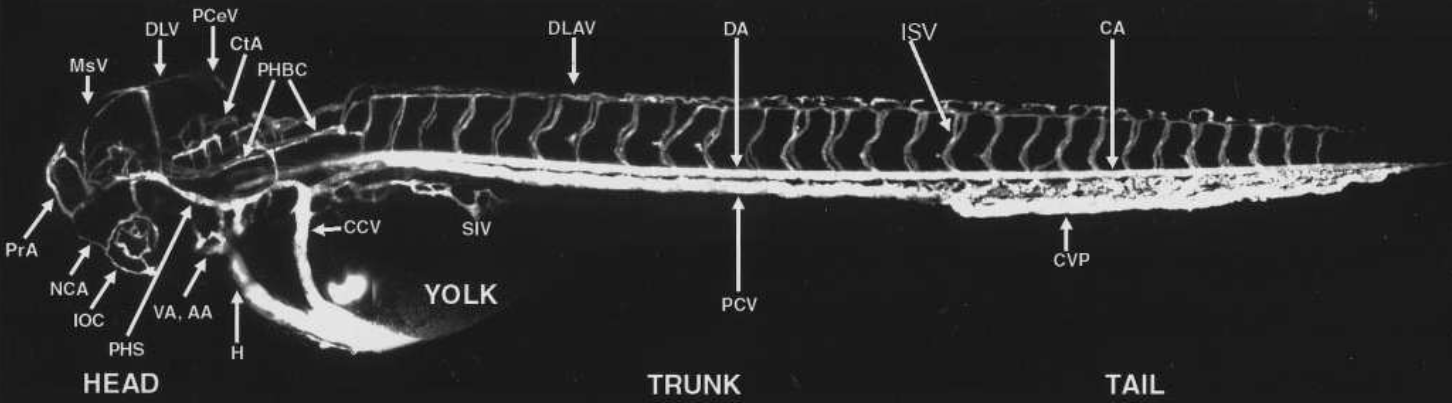
\includegraphics[scale=0.45]{figure/anatomy}
  \end{center}
  \caption[Zebrafish embryo anatomy]{Zebrafish embryo anatomy \cite{isogai01}.}
 \label{anatomy}
\end{figure}
\par

The morphogenesis of the ISV, and CVP involves sprouting, migration, and pruning and can therefore serve as an excellent model for studying angiogenesis.

\section{Challenges}


Current methods analyze images based on intensity and thresholding. These methods perform well on clearly resolved objects against a uniform background but often resort to manual analysis for images that possess information at multiple sizes and heterogeneity across images. To add to the challenge, the images are affected with noise and artifacts. Furthermore, the appearance of zebrafish may vary in intensity, texture, size, and orientation. This problem was brought to attention in a work where zebrafish vasculature became quantifiable only after manual segmentation of the trunk \cite{Tran07}.

Moreover, there is a growing requirement for automated image analysis techniques to process, analyze, and quantify zebrafish images. Meeting such objectives is essential for zebrafish research to reach its full potential in discovery and understanding. Despite the potential of the zebrafish as a model, quantification is still a fledgling field in zebrafish research, primarily due to the lack of tools that can yield objective and quantitative measurements from imaging. From an image processing perspective, a successful algorithm must take into consideration the objectives of the HTS and the content of the images.

All these factors advocate, for automation of as many steps of the analysis as possible. There is an increasing demand for automated image processing to generate quantitative results and to avoid time-consuming manual analysis. According to \cite{Ron13}, the development of dedicated image processing methods has become a serious bottleneck in the full exploitation of the information contained in the acquired image sets. Many custom-made and nongeneric solutions have been developed to answer specific questions. These solutions have an enormous potential to support the analysis of current and future image-based phenotype studies and to avoid parallel developments that tend to \textquotedblleft reinvent the wheel\textquotedblright. We believe that development of a computerized data processing pipeline would be a significant step towards reproducible quantification of phenotypes in large scale or high throughput imaging studies.

Although methods have been developed to process zebrafish images, as the applications of the zebrafish model expands, there is a concurrent demand for a variety of image processing methods. In this work we will focus on the vasculature system of zebrafish, segmenting and developing algorithms for blood vessel development. The vasculature structure is composed of arteries and veins. Blood vessel are highly diverse in length, width, and branching pattern. Significant challenges are associated with blood vessel extraction including, noisy signal, drift in image intensity and poor image contrast.


\section{Research Goal}

%The vascular system is a vital component of all vertebrate animals, supplying oxygen and essential nutrients to everytissue and organ. Zebrafish have a closed circulatory system, and the mechanism of vessel formation are highly similar to those in humans.  It has been suggested that several environmental pollutants could act as vascular disrupting compounds by targeting blood vessel development [3]. A wide range of congenital diseases are associated with blood vessel formation [4], development of the cardiovascular system and associated vascular defects [5], and the adverse effects of exposure to toxic elements during development. 

This work presents a framework of image processing and analysis algorithms that consists of extracting zebrafish, realigning zebrafish embryo images of different orientations, and segmenting, quantifying, and classifying intersegmental vessels (ISV) and caudal vein plexus (CVP). 

Following initial formation of the primitive vasculature by vasculogenesis, most subsequent vessel formation during development takes place via angiogenesis and includes the formation of new vessels by budding growth from, or remodeling of, preexisting vessels. The formation of the ISV and CVP, provides an excellent model for angiogenesis.

ISVs of the trunk are among the first angiogenic vessels to form in all vertebrates. ISVs (fig. \ref{anatomy}) are essential for development and nutrition of the zebrafish embryo. Unlike other vessels, the ISVs are interesting because of the patterned appearance and easy accessibility. Tran et al. \cite{Tran07} has shown that treatment of zebrafish at this early time point had a very strong antiangiogenic effect, causing nearly complete absence of intersegmental vessel growth. The vasculogenic dorsal aorta and posterior cardinal vein were unaffected. Since the intersegmental vessels in zebrafish form by sprouting from the preformed vasculogenic vessels, any compound that disrupts vasculogenesis will also inhibit the growth of angiogenic vessels \cite{Tran07}. All these properties makes ISV one of the most highly investigated vessel in the zebrafish. 

In this work, we have focused on developing an image processing algorithm to automatically segment and quantify ISVs of zebrafish embryos that have been treated by various toxins. The processing pipeline consists of Segmentation, Region Detection, ISV Extraction, ISV refinement, feature quantification and classification. The efficiency of segmentation approach is demonstrated by our experiments of the entire zebrafish vasculature recorded using fluorescence microscopy. The experiments also demonstrate that automated segmentation of ISV is comparable to that of manual segmentation. The quantified features are used to train a linear SVM classifier to identify morphological changes in a dataset consisting of ISV zebrafish embryo images.

Recently, studies have indicated that CVP also undergoes active development, hence providing an additional measure for studying vascular development \cite{Chen05}. The study of the zebrafish CVP and its utilization as a screening assay has not been as prevalent as the ISV, and very few studies have attempted to identify regulators of CVP development. In this work, we study the impact of toxicity on the shape of CVP. Instead of the fine mesh-work of the CVP observed in healthy embryos, treated embryos exhibit the formation of loops in the CVP. %For example, fig \ref{cv} shows the images of healthy and treated zebrafish embryo. 
Previous research has primarily focused on using color, texture \cite{Tran07} and morphological changes \cite{Feng05} for toxicity analysis. Shape information, however, can be another attribute that can be evaluated. A shape descriptor can capture the outline of the shape that other color or texture-based descriptors may not be able to capture.

Hence by quantifying the shape of CVP, and comparing it against that of a healthy embryo, we can identify changes in CVP due to exposure to toxins. Morphological changes due to toxin exposure is modeled based on the proposed gradient weighted co-occurrence histogram of oriented gradients (gCo-HOG). These features are compared to more commonly used histogram of oriented gradients (HOG) features and Co-HOG features that utilizes spatial distribution of neighboring pixels to capture spatial structure. The features are used to train a linear SVM classifier to identify structural changes in a dataset of region of CVP zebrafish embryo images.

We have also presented a study for analyzing effects of Arsenic on overall vasculature development of zebrafish in time-lapse confocal images. We use a transgenic zebrafish that expresses green fluorescent protein (GFP) in the vascular system Tg(Flk1:GFP) to visualize vessel growth in the fish embryo. This transgenic zebrafish line expresses GFP in vascular endothelial cells, which permits real-time imaging of the formation and growth of blood vessels. Time-lapse confocal imaging of embryonic vasculature in the zebrafish is used in conjunction with digital image analysis to monitor and quantify the effect of toxins on vascular development. Imaging captures the dynamics of blood vessel formation over time. In order to quantify these morphological changes, i.e. how much vascular structure has changed over a period of time, it is necessary to compensate for any movements caused by the growing embryo. Thus, in order to record the temporal changes occurring due to vessel growth, it is necessary to establish spatial correspondence between blood vessels that may appear displaced due to embryo movement. Thus quantification of temporal vascular growth can be seen as a problem of image registration. 

The goal of image registration is to align two images, so that common features overlap and differences are emphasized. Image registration has been used widely in the medical field to quantify the influence of changes over time. As an example, registration is required in medicine for comparing computer tomography of patients scan \cite{Betke01}, aligning images from various different modalities to diagnose diseases, etc. Recently, image registration has found application in growth monitoring of tumors and bone \cite{Nielsen97}, \cite{Peter03}. We use a non-rigid registration approach to align images. Non-rigid mapping is based on complete correspondence of images and includes a deformation model as the underlying transformation. We utilize free-form deformation based on B-splines for growth monitoring, and use intensity differences as a similarity measure.

Overall, the methodology presented in this work is quantitative, can be utilized with wide varieties of toxin treated zebrafish, and capable of quantifying changes in fine structure not quantifiable by the human eye. The algorithm automatically processes multiple image files, saves the intermediate image processing results, writes the results in a excel/text format for further statistical analysis. We believe that development of a automated image processing pipeline would be a significant step towards reproducible quantification of zebrafish analysis for HTS. 
%In the past, automatic identification of the applicable region of interes (ROI), and accurate quantification of ROI features has been very challenging.

\section{System Overview}

Zebrafish is a versatile model for vasculature analysis. As its application continues to grow, it is imperative to have an automated image analysis system (fig. \ref{overview}) in place to be able to analyze high throughout data. Obtaining region of interest is the first step for any type of analysis. Multiple zebrafish are imaged in one dish. It is essential to extracts individual zebrafish from image. Our system extracts relevant zebrafish embryo from images. Further, we segment ISV and CVP from embryos. Automated segmentation of ROI opens new opportunities for diversified analysis on zebrafish. 

ISVs are widely used to study toxicology, development, and disease modeling. ISV segmentation is based on multiscale analysis combined with directional information. Multiscale analysis, makes it possible to capture responses from vessels of varying diameter and direction information aids to isolate ISV from other vessels in the region. CVP with its easy accessibility during imaging process, is a potential candidate for research. Realizing its plausible benefits, we have proposed segmentation algorithm based on curvature properties of zebrafish tail.

Although many types of analysis and quantification can be performed on segmented region. Our framework computes morphological properties for quantification of ISV. Shape descriptor is proposed for CVP analysis. Shape descriptor is inspired from Histogram of Gradients. Co-Occurrence of histogram of gradient is combined with gradient information to obtain discriminative representation for CVP region.

Lastly, classification component completes the system. We treat classification as two class binary problem. This system is indicative of healthy embryo vs defective embryo. We demonstrate the validity of our system by analyzing toxin treated data. We used the model to estimate the safe dosage for various chemical. This system can be easily trained to be used for drug modeling, gene expression, etc.

System proposed in this thesis is robust in the manner that each step can be isolated and easily merged with existing or future research. For example, extraction of embryo, ISV and CVP can be effortlessly combined with varied feature extraction methods. 

\begin{landscape}
\begin{figure}[htb] 
 \begin{center}
    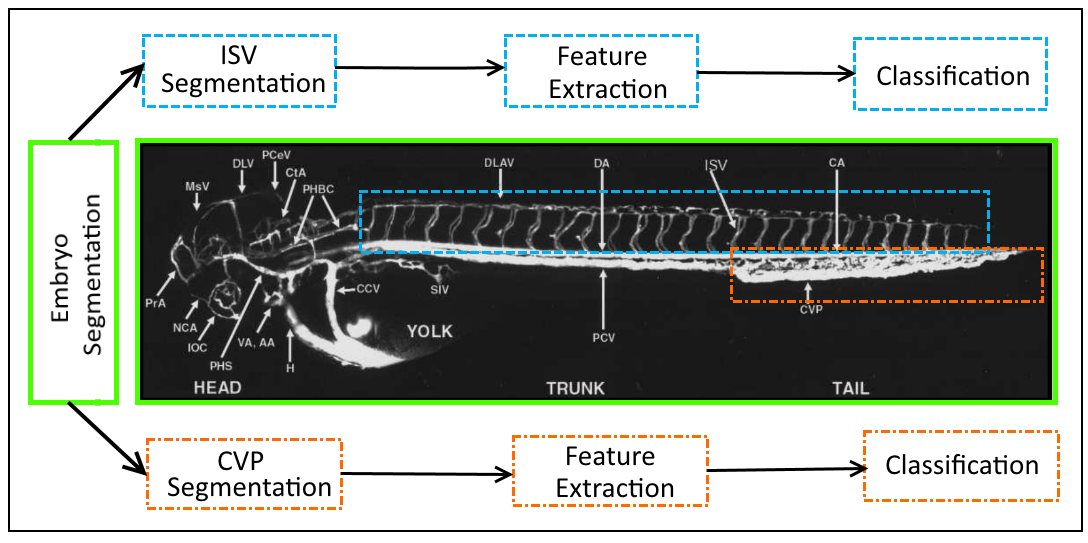
\includegraphics[scale=0.7]{figure/overview.png}
  \end{center}
  \caption[System Overview]{Zebrafish segmentation, feature analysis, classification system}
 \label{overview}
\end{figure}
\end{landscape}



\section{Summary of Contribution}
This thesis studies the image analysis of zebrafish embryo. It makes seven major contributions to this goal:

\begin{itemize}
\item Foremost contribution is the ISV segmentation. There has been many studies indicating viability of using ISV as a model for various application. To our knowledge, automated segmentation of ISV is still largely unstudied problem. In this work we have proposed use of multiscale response and direction information to segment blood vessels.

\item Next is quantification of ISV. We have proposed feature extraction method for ISV morphology, and shown applicability to quantify ISV. Further, we have shown how the features are used for toxicology analysis. 
 
\item Next contribution is segmentation of CVP. CVP is relatively new model as compared to ISV for studying zebrafish. There has been studies showing active molecular development for CVP. Its importance as a model is gaining popularity. CVP segmentation can greatly simplify analysis for HTS. We have proposed an algorithm for CVP segmentation. 

\item In order to utilize shape property of CVP, we have proposed a shape descriptor based on gradient weighted co-occurrence of histogram of gradient. We have proposed to use these descriptors to be able to classify healthy zebrafish embryo, against unhealthy embryos. 

\item We present a toxicology screening system based on lethality rate for ISV and CVP analysis. We used the models derived from morphological properties of ISV and shape properties of CVP to study the effect of increasing dosage on zebrafish in terms of number of zebrafish being impacted with chemicals. Further, this helps us to establish the safe dosage for various chemicals.

\item We studied the vasculature development for time lapse data. This work focuses on capturing temporal vasculature changes in zebrafish. This can work as an initial pass for studying changes in zebrafish development under the influence of chemicals. We have shown utilization of developed algorithms to study arsenic treated zebrafish embryo. 

\item Lastly, the work-flow presented in this thesis is fully automated. The segmentation and analysis of the imaging data is one of the most challenging tasks in automation of the zebrafish applications. Due to lack of robust solutions for this problem, most of the analysis is currently being performed manually. This serves as a huge bottleneck for interpreting data from HTS.

\end{itemize}

\section{Thesis Outline}
The remaining chapters are organized as follows:

\begin{itemize}

\item Chapter \ref{chap:RelatedWork} gives the detail about related work. Related work is clustered according to type of analysis ( automated vs manual).

\item Chapter \ref{chap:seg} presents segmentation algorithm for zebrafish embryo, ISV and CVP. Embryo segmentation is based on region and moment analysis. ISV segmentation uses multiscale property with directional information. CVP segmentation is based on curvature analysis.
 
\item Chapter \ref{chap:feature} describes the features used for quantification of ISV and CVP. We describe our propose algorithm utilizing gradient information with co-occurrence matrix of histogram of gradient. Also, we will discuss time lapse vasculature quantification. 

\item Chapter \ref{chap:results} summarizes approach and our results. We will present results for ISV segmentation, comparing proposed segmentation with manual segmentation. We will also present a classification system for ISV (healthy vs unhealthy), based on its morphological properties. We will also present result for classification system  based on shape properties of CVP. We will describe the toxicology screening system based on modeling ISV and CVP, and how it can be used to derive safe dosage.

\item Lastly, chapter \ref{chap:conclusion} concludes the thesis. We discuss limitations of the work and give guidelines for future work.

\end{itemize}

\chapter{Related Work}\label{chap:RelatedWork}

Utilization of zebrafish as a model has received lots of attention in recent year. Advances in imaging technologies and growing number of applications is pressing the need for automated image analysis methods. Table \ref{table:reviewPast} presents the summary of past work for zebrafish analysis. We divided the related work into three sections on the basis of analysis: manual; semi-automated and automated. We further grouped the automated methods based on the type of methods used for analysis.

\section{Manual Analysis}

Arslanova et al. \cite{Arslanova10} developed a method to examine live zebrafish that were each treated with gamma-secretase inhibitors (GSI), DAPT {N-[N-(3,5-difluorophenacetyl-L-alanyl)]-S-phenylglycine t-butyl ester}, Gleevec, or fragments of Gleevec in a zebrafish model of Alzheimer's disease (AD). 


\begin{landscape}
\begin{table}
\caption{Summary Zebrafish Image Analysis} % title name of the table
\centering % centering table
\scalebox{0.85}{
\begin{tabular}{| l | l | l | l | l | l | l |} % creating 10 columns
\hline\hline % inserting double-line
 \textbf{Method} & \textbf{Imaging Modality} & \textbf{Anatomy} & \textbf{Dimension} & \textbf{Application} & \textbf{Analysis Type} & \textbf{Year}
\\ [0.5ex]
\hline % inserts single-line
% Entering 1st row
    Liu et al. & Digital Microscopy & Whole Organism & Gene Expression & 2D & Automated & 2006 \\ \hline
		
    Shirinifard et al. & Confocal & Vasculature & 3D + t & Toxicology & Manual & 2013 \\ \hline
		
		Chen et al. & n.s. & Vasculature & 2D & Gene Expression & Manual & 2005 \\ \hline
		
		Liu et al. & Bright Field & Whole Organism & 2D  & Toxicology & Automated & 2012 \\ \hline
		
		Xu et al. & Bright Field & Torso & 2D & Toxicology & Automated & 2010 \\ \hline
		 
		Arslanova et al. & Microscope & Whole Organism & 2D & Gene Expression & Manual & 2010 \\ \hline
		
		Tran et al. & Fluorescent & Vasculature & 2D & Drug Discovery & Semi Automated & 2007 \\ \hline
		
		Yozzo et al. & Fluorescent & Whole Organism & 2D & Toxicology & Semi Automated & 2013 \\ \hline
		
		Stern et al. & Microscope & Whole Organism & 2D & Toxicology & Automated & 2011 \\ \hline
		
		Kato et al. & CCD Camera & Whole Organism & 2D + t & Behavior pattern & Automated & 2004 \\ \hline
		
		Vogt et al. & Fluorescent & Vasculature & 2D & Toxicology & Automated & 2009 \\ \hline
		
		Feng et al. & Fluorescent & Vasculature & 3D & Toxicology & Automated & 2005 \\ \hline
		
		Chen et al. & Microscope & Whole Organism & 2D & Drug Discovery & Automated & 2011 \\ \hline
		
		Tal et al. & Confocal & Whole Organism & 3D + t & Toxicology & Semi-Automated & 2014 \\ \hline
		
		Kamali et al. & Confocal & Brainstem & 3D & Disease Modeling & Automated & 2009 \\ \hline
		
		Anilla et al. & Fluorescent & Whole Organism & 2D & Disease Modeling & Semi - Automated & 2013 \\ \hline
		
		Mccollum et al. & n.s & Whole Organism & 2D & Toxicology & n.s. & 2011 \\ \hline
		
		Alshut et al. & Microscope & Whole Organism & 2D & Toxicology & Automated & 2010 \\ \hline
		
		Peravali et al. & Microscope & Brain & 2D & n.s. & Manual & 2011 \\ \hline
		
		Bang et al. & CCD Camera & Whole Organism & 2D + t & Behavior pattern & Automated & 2002 \\
		
\hline % inserts single-line
\end{tabular}
\label{table:reviewPast}
}
\end{table}
\end{landscape}

Several GSI are in clinical trials for the treatment of AD. Brain regions (ROI) from the dorsal view images are manually segmented. The intensity of each ROI is quantified. To measure the gene expression, a manual approach is not only time-consuming but also lack objectivity due to inter-observer variations.

Shirinifard et al. \cite{Shirinifard13} discussed quantitative analysis of growth dynamics for characterization of both normal and perturbed growth for ISV. Their method is based on analyzing ISV trajectories (sequences of successive 3D locations over time). Manual Tracking plugin in FIJI ImageJ is used to track 3D position of ISV sprout bases and tips over time (x, y, z coordinates over time). ISV sprout base position is the midpoint of the sprout where it intersects with the DA. ISV tip position is the farthest point on the ISV from the point of attachment on DA. Displacement and angle between the ISV and the DA is used to correct for zebrafish embryos twitching. Average trajectories are calculated for control and for arsenic treated embryo. Average trajectories are fitted with quadratic curve to produce a canonical ISV trajectory.  Curvature, average directed migration speed and directionality were computed from canonical trajectories. Curvature, average directed migration speed and angle between the ISV and DA were different for arsenic treated vs untreated.

Chen at al. \cite{Chen05} proposed to use caudal vein to study the affects of modifications of sulfate 6-O sulfotransferase (HS6ST) genes on zebrafish development. Authors observed formation of large loops with high penetrance for the caudal vein. Quantification is done on the basis of number of embryos showing abnormal caudal vein development. 

In the review done by Mccollum et al. \cite{mccollum2011} explores the questions of using zebrafish as a screening tool for human risk assessment. Toxicity effects on the zebrafish development are reviewed from existing literature. Toxic effects are reported on cardiovascular, somite, muscular, skeletal, and neuronal systems. They also report abnormal behavior, changes in gut, pancreas, liver, and kidney development, as well as toxic effects on the immune system and lipid metabolism. 

Cheng et al. \cite{cheng2001} studied the effects of cadmium on cardiovascular development in zebrafish embryos. They concluded that exposure to cadmium could affect the morphogenesis of the vasculature. In embryos with visible abnormalities, the vasculature in the malformed region correlated well with defective vascular patterning. There is a significant reduction in number of branches for cadmium exposed embryos as compared to health embryos.  


\section{Semi-Automated Analysis} \label{sec:RelatedWorkSemi}

Tran et al. \cite{Tran07} proposed an interactive algorithm using the Discovery-1/MetaMorph software to rapidly analyze each image. ISV is isolated from rest of images, by manually removing trunk from the fluorescent image. ISV is separated from rest of image using mask. The software counts the number of intersegmental vessels and branching arteries in the isolated trunk of the embryo. Manual segmentation of trunk restricts its usage for HTS. As shown in our work certain compounds do not alter ISV count but, end up changing other dynamics of ISV.

Yozzo et al. \cite{Yozzo13} screened 10 known cardiovascular toxicants through an image analysis pipeline that included ISV sprout length quantification. Semi-automated methods are used to isolate regions of interest and quantify heart rate, circulation, pericardial area, and intersegmental vessel area, whereas a fully automated method is used to quantify body length.

Tal et al. \cite{Tal14} tested the effect of environmental chemicals on formation of the vascular system. They developed a quantitative assay in transgenic zebrafish and evaluated the assay using angiogenesis inhibitors that target VEGFR2 (PTK787) or EGFR (AG1478). Both PTK787 and AG1478 exposure impaired ISV sprouting, while AG1478 also produced caudal and pectoral fin defects at concentrations below those necessary to blunt ISV morphogenesis. The functional consequences of vessel toxicity during early development included decreased body length and survival in juvenile cohorts developmentally exposed to inhibitor concentrations sufficient to completely block ISV sprouting angiogenesis. Vascular growth depicted in time-lapse image stacks is quantified in automated manner where as ISV length is manually observed. 

ZebIAT is image analysis tool developed by Anilla et al. \cite{annila2013} that allows both automatic or semi-automatic registration of the outer contour and inner organs of zebrafish embryos. ZebIAT provides a registration at different stages of development and an automatic analysis to study cancer progression. The user manually marks the organs or other areas of interest in the reference zebrafish embryo image. Outline of the zebrafish is obtained by segmentation and edge detection. Landmark based registration is applied to register images to reference image. Labeled cancer cells are detected using a method of multiscale product of wavelet and the mean fraction of the area of each organ that exhibited cancer spots in the embryos is examined.

To enable large scale observations Peravali et al. \cite{peravali2011} developed an algorithm to identify head region from low resolution image based on template matching. The regions of interest are subsequently imaged automatically at high magnification, enabling rapid capture of cellular resolution data. The pixel location in the source image yielding the largest normalized cross-correlation measure was considered the best match between the template and the source image, and is chosen as the center of the field of view for subsequent high-resolution imaging.

\section{Automated Analysis}
This section discuses automated techniques for zebrafish image analysis. Review is grouped into various subsection, based on type of method used for image analysis. Figure \ref{overviewRelatedWrok} gives an overview of algorithm utilized for analysis. It also includes, few of the methods described in section \ref{sec:RelatedWorkSemi}.

\begin{landscape}
\begin{figure}[htb] 
 \begin{center}
    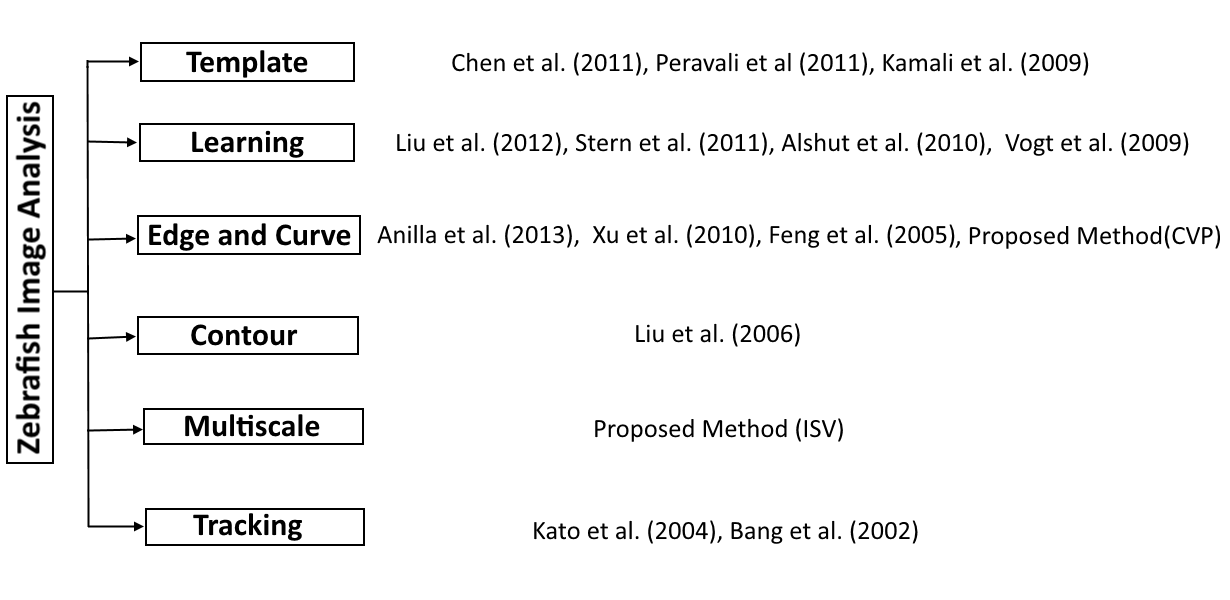
\includegraphics[scale=0.6]{figure/review.png}
  \end{center}
  \caption[Overview of an automated/semi-automated image analysis methods.]{Overview of an automated/semi-automated image analysis methods.}
 \label{overviewRelatedWrok}
\end{figure}
\end{landscape}
\par

\subsection{Template Based}

Chen et al. \cite{Chen11} proposed a robust automatic segmentation to identify ROIs for gene expression quantification. Their pipeline consisted of image alignment, segmentation, extraction and quantification of 15 ROIs. The telencephalon, left and right (L\&R) dorsal diencephalon, L\&R olfactory vesicles, ventral midbrain, L\&R retina, L\&R branchial arches, ventral hindbrain, L\&R dorsal hindbrain, and L\&R pectoral fin is quantified to evaluate gene expression. Size of each of the ROI is calculated for quantification. 

Kamali et al. \cite{kamali2009} developed a 3D template-based tracing algorithm to localize and differentiate the fluorescent neurons. A control template consisting of 28 zones with 14 zones on each side of the brainstem is created as a representation of 300 neurons that descend from the larval zebrafish brain into the spinal cord. The template is initialized by registering neurons manually identified in the different zones. After the creation of the template, image processing steps are applied to detect neurons and assign them to the template. First process is image registration of confocal z-stacks into a normalized space. User select three points on a MIP projection of confocal z-stack and corresponding points on template. Affine transform is applied to the 3D image stack to register it to the template. Second process of segmentation involves two steps: (1) neurons are segmented on each xy - plane to find a set of intensity contours with appropriate size and shape so as to reveal each neuronal cell body present in the plane (2) segmented results over consecutive xy-plane images are associated with the same neurons based on the assumption that each neuron spans several images along the z-direction. Lastly, for cell identification template is used in conjunction with the segmented boundary contours to assign detected neurons to specific zones and sub-zones of the brainstem.

\subsection{Learning Based}

Liu et al. \cite{Liu12} proposed a recognition model for high throughput screening of toxicity based on image descriptors based on color and texture combined with a support vector machine to recognize three basic phenotypes (hatched, unhatched, and dead). The best performing model is attained with three image descriptors (color histogram, representative color, and color layout) identified as most suitable from an initial pool of six descriptors. The SVM classification model is developed using the three descriptors: (a) Global and Semi-global Edge Histogram Descriptor (GSEHD), (b) Representative Color Descriptor (RCD), and (c) Color Histogram Descriptor (CHD). They reported an average classification accuracy of 97.40±0.95\% in a 10-fold cross-validation and 93.75\% classification accuracy for a stress test with zebrafish images of low quality. This system can be used to identify extreme cases of toxicity, but further analysis is needed to identify less extreme cases.

Alshut et al. \cite{alshut2010} proposed learning based classification approach, which detects the embryo in the well, classifies its status and derives characteristic parameters for the regions. Expert labeled the data to the classes dead, alive or unknown. Chorion is segmented from background using adaptive threshold and features are derived based on intensity edge filter, and chorion size. Two most discriminative features are selected by MANOVA (multivariate analysis of variances). Using these two features, the classification is performed utilizing a Bayesian classifier.

Stern et al. \cite{Stern11} focused on automatically detecting specific interest points in microscopy images. Images are manually annotated by expert to identify interest points coordinates and to train models able to predict those interest points in new, unseen images. The approach first extracts sub-windows (or patches) around points of interest and at other randomly chosen positions within images. The patches are described by various visual features, RGB, HSV, Grayscale, Edge strength, Local Binary Pattern. A classification or a regression model is built using these features. In the classification scheme, the model is trained to predict whether the central pixel of a sub-window is an interest point or not (a binary classification problem). In the regression scheme, the model predicts the distance between the central pixel of a sub-window and the interest point.

Vogt et al. \cite{Vogt09} implemented a user guided image interpretation tool to generate rule-based hierarchical image segmentation. The zebrafish embryos are first segmented, and the large vessels and head structures are identified based on pixel values. The algorithm then removes small and isolated objects. Next, the remaining regions are re-processed to identify the head, dorsal aorta, and posterior cardinal vein. These pre-processed images were then used for blood vessel quantification. Numerical measurements of blood vessels development such as area, length, and shape are captured. 

\subsection{Contour Based}

Liu et al. \cite{Liu06} have proposed to automatically quantify the neurons and somites in a large number of zebrafish images, as well as quantitative measurement of gene expression levels in zebrafish embryos. Neurons are segmented from edge image using circular Hough transform. Rohon–Beard (RB) sensory neurons are segmented using method based on intensity projection. Somites are recognized using gray level co-occurrence matrix, and edge direction histogram. ROI for genes quantification is established with region growing segmentation. Neurons quantification is based on its count. There is neuron loss in zebrafish embryos due to knockdown of AD-linked genes. Somites are quantified using features extracted from gray level co-occurrence matrix for detection of defective somites.

\subsection{Curvature and Edge Based}

Xu at al. \cite{Xu10} proposed an algorithm focused on detecting and quantifying pigments in zebrafish embryos. They automatically identify torso area through series of image processing steps. Steps include, finding single zebrafish in an image and then rotating the images so the embryo is positioned with its head region to the upper right corner and with its back pointing upward and abdomen downward to allow the algorithm to search the abdominal region based on the zebrafish anatomy. A watershed method is used to remove the head region from the torso that contains the pigmentation. Otsu’s method is applied on the torso for segmentation, which is quantified and used for toxicology. 

Feng et al. \cite{Feng05} developed a 3D attributed vessel represent graph (AVRG) approach to reconstruct caudal vasculature of zebrafish embryo. The major steps of the framework include pre-processing, vasculature reconstruction, vascular structure quantification, and presentation. Pre-processing steps for vessel segmentation include: (1) Image enhancement; (2) Adaptive thresholding; (3) Vessels registration; (4) Edge tracking and curve fitting. The cross-sections of a segmented vessel are represented by ellipses. The surface of a blood vessel is represented by triangle meshes. Vasculature structure is reconstructed by locating junction points at the intersections of two or more vessels. Reconstructed vasculature structure is then utilized for quantification of the number and connectivity of the vessels, their size, length, and volume, as well as the distance between any two vessels.


\subsection{Tracking Based}

Bang et al. \cite{bang2002} developed an automated screening assay to detect hearing defects in zebrafish by monitoring their behavior after receiving a loud sound burst. The image was acquired immediately before the tone burst was subtracted from the image acquired immediately after the tone burst. If the zebrafish did not respond to the tone burst, due to hearing defects, the subtraction of its images produced an image approximating zero. If the zebrafish responds to the tone burst by moving to a different position, the subtraction result contains both positive and negative pixel values that can be detected by taking the absolute value of the resulting image and segmenting it by an appropriate threshold.

Kato et al. \cite{Kato04} developed computer image processing system for quantifying zebrafish behavior. Zebrafish images were extracted in real time from the original image as a binary image by removing a background of the aquarium before the fish are introduced. To maintain an effective frame rate that is high enough to capture the movement of the zebrafish, skipping search method is applied on data. In each frame, only one fourth of the pixels are \textquotedblleft skippingly\textquotedblright examined, and then only the areas of interest that are recognized as zebrafish are analyzed in more detail in the two diagonal directions and in two crosswise directions with a continuous search. Chasing behavior of pairs of fish are quantitatively analyzed based on the positional coordinates of their center of gravity.

\begin{figure}[htb] 
 \begin{center}
    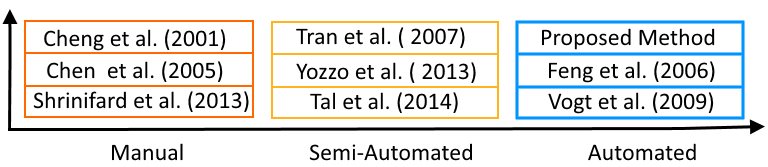
\includegraphics[scale=0.65]{figure/analysisReview.png}
  \end{center}
  \caption[Overview of vasculature image analysis methods]{Overview of vasculature image analysis methods.}
 \label{analysis}
\end{figure}

\begin{figure}[htb] 
 \begin{center}
    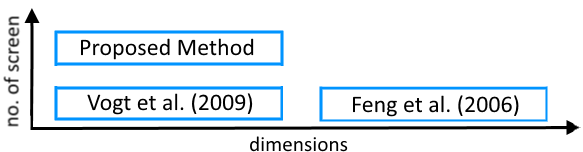
\includegraphics[scale=0.85]{figure/automatedReview.png}
  \end{center}
  \caption[Overview of an automated vasculature image analysis methods]{Overview of an automated vasculature image analysis methods.}
 \label{automated}
\end{figure}



\par
Automated analysis of vasculature is still a budding field. Feng \cite{Feng05}, and Vogt \cite{Vogt09}, and proposed method are the only studies dedicated to automated analysis of vasculature blood vessel (fig. \ref{analysis}).  The work presented in their papers has been performed on limited number of compounds (fig. \ref{automated}); there is still a question about its scalability. Feng \cite{Feng05} performed 3d reconstruction of few vessels, where in our work we capture the dynamics of all ISVs. In this work, we have proposed a segmentation and quantification algorithm for ISV and CVP. Segmentation is a very crucial and important step for any kind of analysis. Interestingly, an automatic segmentation of ISV and CVP is still an untouched problem. Segmentation based either on thresholding or on edge detection of images are not sufficient to analyze ISV. ISV are highly diverse; they differ in size, shape, intensity, and occluded with noise. The orientation and amount of details of each embryo are different. One image has multiple embryos placed in various orientations. %(Show image for data issue0) 
To quantify different regions, manual analysis requires one to draw ROIs for every image and then measure the features in each ROI. Often a human observer needs to rotate the images to the same orientation before drawing ROIs and quantifying pixel intensity, making their laborious work more tedious. In addition, manual analysis is subject to inter-observer variation and lacks repeatability.
\par
In summary, although methods have been developed to process zebrafish images, as the applications of the zebrafish model expands, there is a demand for a variety of automated image processing algorithm. In this work we have presented a techniques and a framework for segmentation, representation, quantification and classification of the zebrafish ISV and CVP from  images. The methodology presented is quantitative, can be utilized with wide varieties of toxin treated zebrafish, and capable of quantifying changes in fine structure not quantifiable by the human eye. Relevance of our work is further amplified, by having a model to be able to determine safe dosages for assays of compounds. In next few chapters we will present detailed description of our approach.


\chapter{Zebrafish Segmentation}\label{chap:seg}
Zebrafish vessel segmentation can be utilized for delineation of morphological attributes of blood vessels, such as length, width,
area and/or angles for disease modeling, drug screening, toxicology, and gene expression evaluation. Automated segmentation can help screen larger populations for vessel abnormalities. In this chapter we will describe segmentation algorithm for zebrafish embryo, its ISV and CVP.

\section{Embryo Segmentation}
\begin{figure}[htb] 
 \begin{center}
    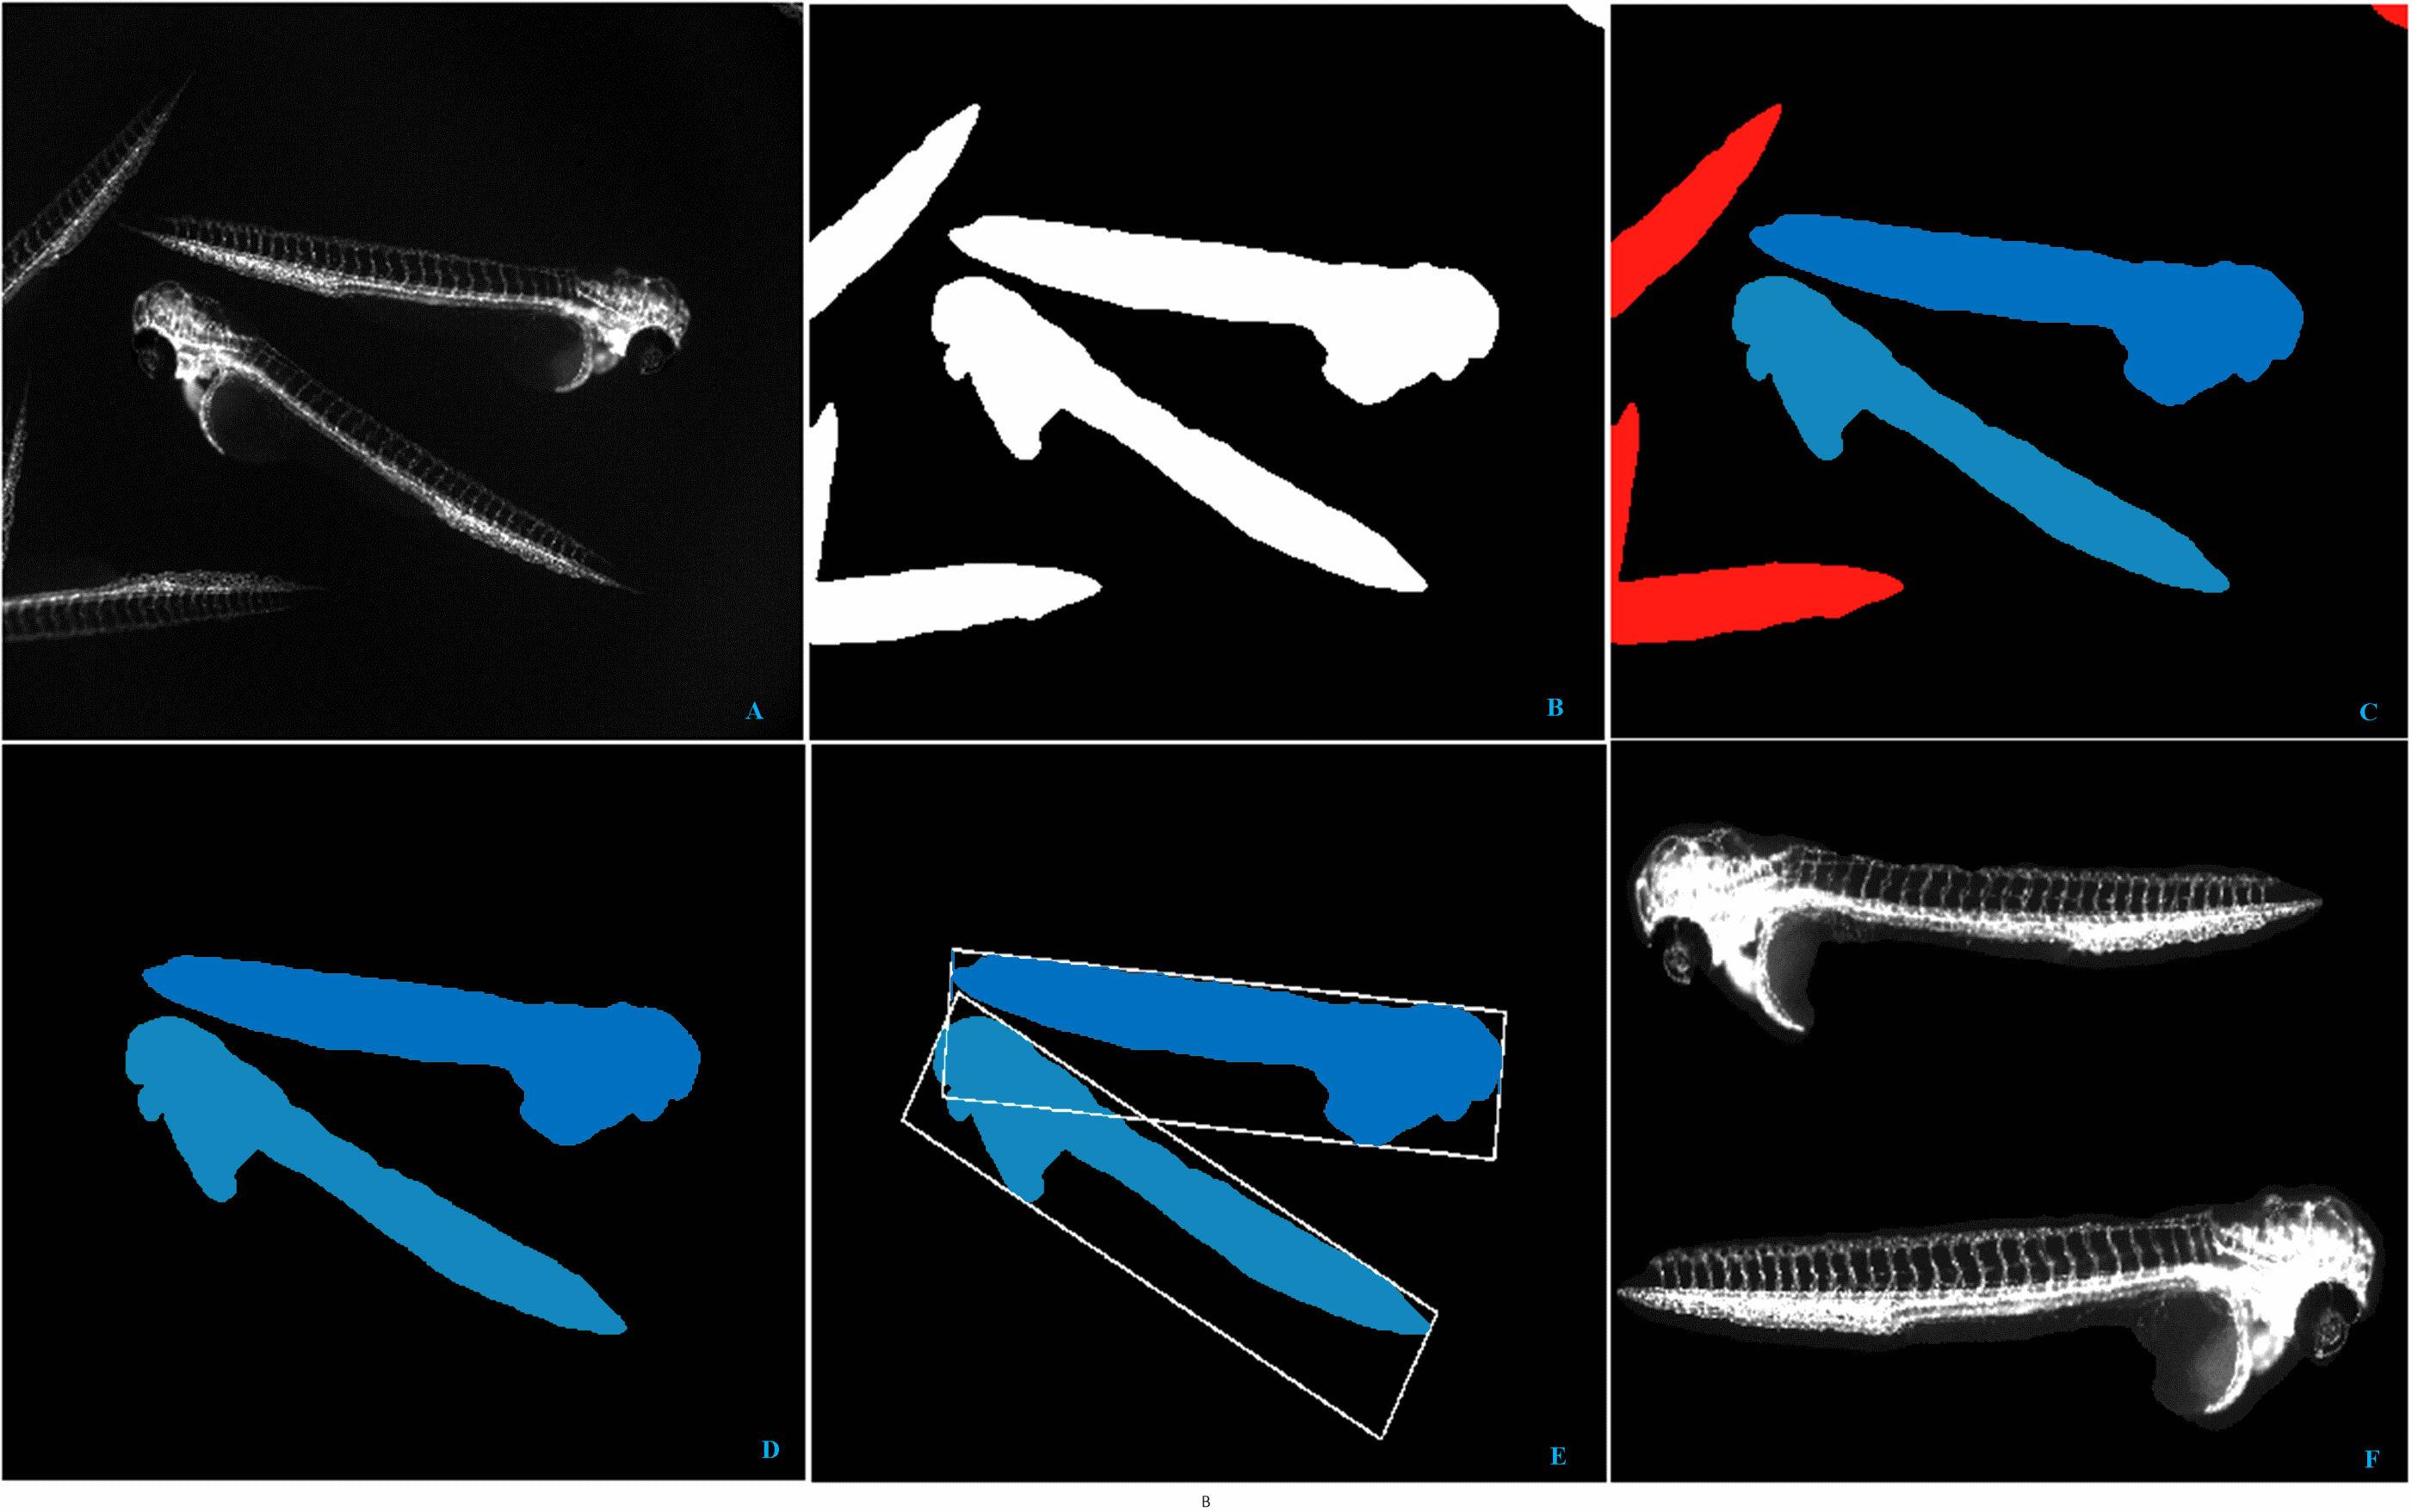
\includegraphics[scale=0.25]{figure/wholeEmbryo.png}
  \end{center}
  \caption[Zebrafish embryo extraction procedure]{Figure \ref{EmbryoSeg}A, \ref{EmbryoSeg}B shows multiple embryos in an image, and corresponding segmented image. In fig. \ref{EmbryoSeg}C embryos shown in red are outliers and in blue are valid embryos. After extracting the relevant embryo, we rotate each embryo by an angle that major axis of bounding box makes with the horizontal axis. If bounding box intersect, we choose the largest connected component.}
 \label{EmbryoSeg}
\end{figure}

An image may have multiple zebrafish embryos as shown in fig. \ref{EmbryoSeg}A. Our aim is to capture the complete anatomic structure of each zebrafish. Due to the limited resolution of a microscopic image, adjacent objects may appear to be touching, each other or boundaries. The algorithm presented detects the valid zebrafish embryos in an image and excludes rest. For, this we smooth the image with Gaussian filter. 
Smoothing reduces the finer details of an embryo, hence producing a uniform foreground (zebrafish embryo) against uniform background.  The background and the foreground are separated, hence we can perform thresholding with triangle method \cite{zack77}. The method is based on a histogram of image intensities. The triangle method constructs a line between the histogram peak and the farthest end of the histogram. The threshold is the point of maximum distance between the line and the histogram. 
%\begin{comment}

Thresholding is followed by connected component labeling for extracting the each of the zebrafish embryos. Let $C_{i}, i = 1,2,\ldots, n$ be the labeled component sets in an image $I$ with size $w\times h$. In each connected set, let the labeled pixels be given by $C_{i} =  ((x_{ij}, y_{ij}), j= 1,2,\ldots, m)$. 
Since in each image we are looking for a complete anatomic structure, we discard labeled component $C_{i}$ in $I$ under 3 conditions (fig. \ref{EmbryoSeg}(c)): 
\\*(i) if blobs are touching the boundaries of image. 
%\begin{equation}\label{eq:cond1} (x_{ij} == w || y_{ij}  == h ||x_{ij} == h || y_{ij}  == w), j \in (1,2,\ldots, m)\end{equation}
\\*(ii) if number of labeled pixels in connected set is above certain threshold  
%\begin{equation}\label{eq:cond2}size(C_{i}) > upper\end{equation}
\\*(iii) if number of labeled pixels in connected set is below certain threshold. 
%\begin{equation}\label{eq:cond3}size(C_{i}) < lower\end{equation}

\begin{equation}
C_{i} = \begin{cases} 0, &\mbox{if } (x_{ij} == w || y_{ij}  == h ||x_{ij} == h || y_{ij}  == w) j \in (1,2,\ldots, m) \\
0 & \mbox{if } size(C_{i}) > upper \\
0, & \mbox{if } size(C_{i}) < lower \\ 
255, & \mbox{if } otherwise. \end{cases}  
\end{equation}

where, upper and low are calculated based on the dataset. Values for upper and lower is easy to estimate. Upper is approximately $1.5$ times, and lower is $\frac{1}{3}$ of the average size of zebrafish embryo.

As the orientation of zebrafish embryo varies in the image, the next step of extraction will use the shape information of the embryo. The position of the zebrafish embryo in the image is normalized, to place longest axis of fitted ellipse parallel to horizontal axis. Moment invariants allow us to find the best fitting ellipse for a target object. 
For an image I, the moment of order $(p + q)$ is defined as:

\begin{equation}
%m_{pq} = \[ \int\limits_{-\infty}^{+\infty}  \int\limits_{-\infty}^{+\infty} x^p y^q I(x,y)dxdy.\]
m_{pq} = \int\limits_{\vphantom{b}{-\infty}}^{\infty} \int\limits_{-\infty}^{\infty} x^p y^q I(x,y)\mathrm{d}x \mathrm{d}y 
\label{eq:moment1}
\end{equation}
$p,q = 1,2,\ldots$

We can simplify Eq. \eqref{eq:moment1} further,
\begin{equation} 
m_{pq} = \sum_{p}\sum_{q} x^p y^q
\label{eq:moment2}
\end{equation}
$p,q = 1,2,\ldots$

To further reduce Eq. \eqref{eq:moment2}  over a connected region $C$, in an image:

\begin{equation} 
m_{pq} = \sum_{C} x^p y^q
\label{eq:moment3}
\end{equation}
$p,q = 1,2,\ldots$

Let $(x_{c}, y_{c})$ be the centroid of region C. The central moments are defined as:

\begin{equation}
\mu_{pq} = \sum_{C} (x - x_{c})^p (y - y_{c})^q
\end{equation}

From the eq.\eqref{eq:moment3}, $m_{00}$, gives the area of C. The centroid $c = (x_{c}, y_{c})$ and angle $\theta$ between the largest axis and the x-axis can be calculated as follows:

\begin{displaymath} x_{c} = \frac{m_{10}}{m_{00}}\end{displaymath}

\begin{displaymath}y_{c} = \frac{m_{01}}{m_{00}}\end{displaymath}

\begin{equation}
\theta = \frac{\arctan(\frac{b}{a-c})}{2}
\end{equation}

where a, b, c cane be defined as:

\begin{displaymath}a = \frac{m_{20}}{m_{00}}  - x_{c}^2\end{displaymath}

\begin{displaymath}b = 2(\frac{m_{11}}{m_{00}}  - x_{c}y_{c})\end{displaymath}

\begin{displaymath}c = \frac{m_{02}}{m_{00}}  - y_{c}^2\end{displaymath}

Connected components are rotated around its $c = (x_{c}, y_{c})$, with the angle $\theta$ (fig. \ref{EmbryoSeg}D). Since the mask obtained likely contains small connected components, we find the relevant embryo by selecting the largest connected component in the mask. The steps are exemplified in fig. \ref{EmbryoSeg}D, \ref{EmbryoSeg}E.

\section{Region of Interest Detection}\label{sec:roi}
After isolating zebrafish embryo's complete anatomical structure, we proceed to detect region of interest (ROI). We are interested in ISV and CVP region. We bisect zebrafish into ISV + DLAV region and tail + head region. The vessels dorsal aorta, tail and head structure have high intensity value, as they are large in size, and tightly knit together. On the other hand, ISV and DLAV are very thin and located at distance, this results in ISV and DLAV to having low intensity as compared to large vessels as depicted in fig. \ref{intensityProfile}.

\begin{figure}[htb] 
 \centering
    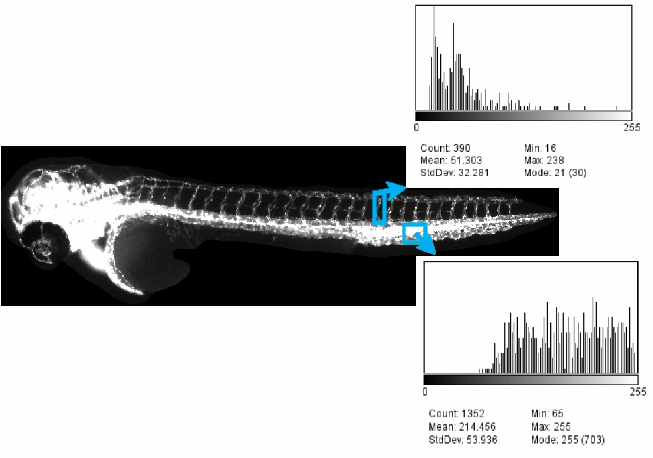
\includegraphics[scale=0.3]{figure/intensityProfile.png}
  \caption[Intensity profile of ISV + DLAV region compared to tail + head region]{The difference in intensity profile of ISV + DLAV region compared to tail + head region. The difference in intensity profile average value is more than 150.}
  \label{intensityProfile}
\end{figure}

We enhanced contrast, to further exemplify differences in their intensity value. Intermodes threshold based on bimodal distribution is well suited for separating ISV + DLAV from rest of embryo. The histogram is smoothed using a running average of size 3, until there are only two local maxima. The threshold value is the average of two peaks. 

\begin{figure}[htb] 
 \centering
    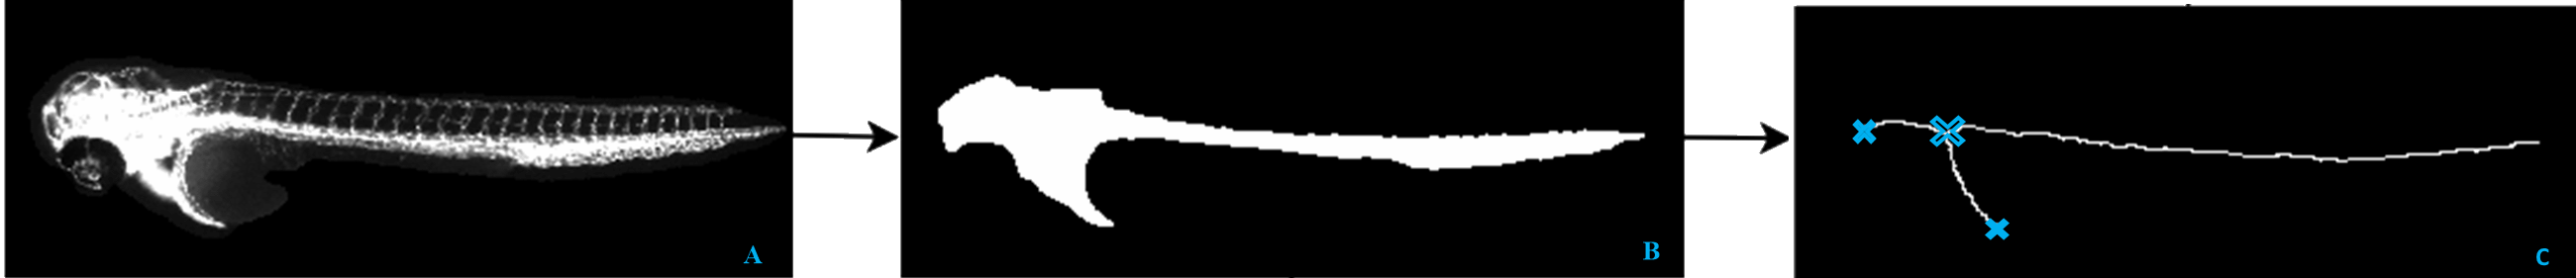
\includegraphics[scale=0.25]{figure/headYolkPosition.png}
  \caption[Procedure for finding head yolk position]{ Procedure for finding head yolk position. Figure \ref{noiseRem}B is obtained by masking out ISV + DLAV region from fig. \ref{noiseRem}A. Skeleton (fig. \ref{noiseRem}C) of mask is used to find the position of head and yolk and point of intersection of head and yolk region, and hence remove the rest of data.}
  \label{noiseRem}
\end{figure}

\begin{figure}[htb] 
\centering
    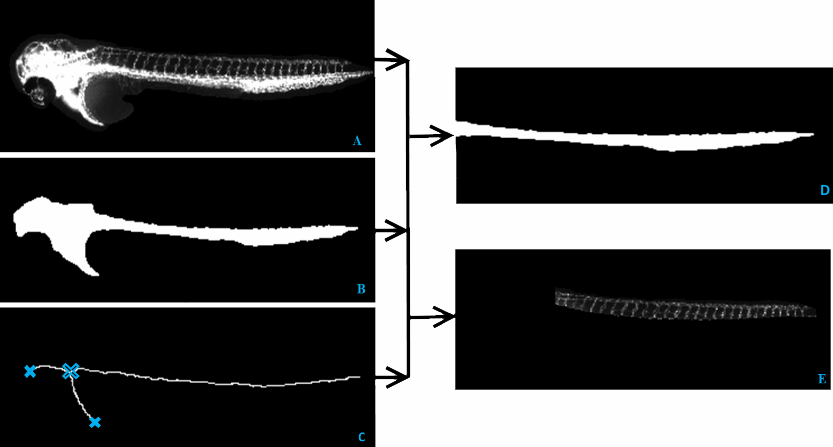
\includegraphics[scale=0.65]{figure/isvCvpRegion.png}  
  \caption[ROI Detection]{Procedure for extracting ISV + DLAV region and tail region. Figure \ref{region}D is obtained by masking segmented region shown in fig. \ref{region}b and removing head region. Figure \ref{region}E is obtained by masking out segmented region fig. \ref{region}B from \ref{region}A. Figure \ref{region}C is used to remove isolated region from head and yolk.}
  \label{region}
\end{figure}

Although above step separates zebrafish embryo into two region. But there is still some isolated portion of head, and yolk region left to be masked out. Specifically for tail + head region, we want to mask out only tail region. Skeleton of segmented image is used to find head, and yolk position. We can have two possibilities for head and yolk. Head can be on right side of image (fig. \ref{noiseRem}D) or left side of image. Yolk can face up or upside down (fig. \ref{noiseRem}D). We scan the skeleton image from top (from origin) along image width and store pixel values in pixelLocUp. Similarly, we scan the skeleton image from bottom (from height) along image width and store pixel values in pixelLocDown. Next we compute the euclidean distance between each pair of entries in pixelLocUp, and pixelLocDown as described in algorithm ~\ref{alg:cleanImage}. Next step is to find the position of yolk, if yolk is facing up or upside down (algorithm ~\ref{alg:yolkLocation}). Lastly for finding head location we use steps described in algorithm ~\ref{alg:headLocation}.

\begin{algorithm}
  \caption{Algorithm for finding distances between skeleton point from top and bottom.}
  \begin{algorithmic}
	\For  {$i=1$ to $height$} 
	\For  {$j=1$ to $width$} 
	\If {($Image(i,j) == 255$)}
			 \State  $pixelLocUp = [pixelLocUp; i j]$
			\State break
    \EndIf  
	\EndFor
	\EndFor
	\For  {$i=height$ to $1$} 
	\For  {$j=width$ to $1$} 
	\If {($Image(i,j) == 255$)}
			\State  $pixelLocDown = [pixelLocDown; i  j]$
			\State break
  \EndIf  
	\EndFor
	\EndFor
		
 \LineComment{pairwise Euclidean distance for pixelLocUp, pixelLocDown}
 \State pixelLocUpDist = dist(pixelLoUp, pixelLocUp)
 \State pixelLocDownDist = dist(pixelLocDown, pixelLocDown)
\end{algorithmic}
\label{alg:cleanImage}
\end{algorithm}

\begin{algorithm}
  \caption{Algorithm for finding yolk position, and cleaning region containing yolk }
  \begin{algorithmic}
 \LineComment{Yolk is facing up}
 \If {($max(pixelLocUpDist) > max(pixelLocDownDist)$)} 
    \State $top =  true$
    \State $location =  find(pixelLocUpDist == max(pixelLocDist))$
\LineComment{Yolk is facing down}
 \Else
   \State $top =  false$
   \State $location =  find(pixelLocDownDist == max(pixelLocDownDist))$
\EndIf 
\LineComment {clean image above pixelLocUp}
\If {( $top == true$ )}
	\For {$i = 1$ to $pixelLocUp.size$}
		\For {$j = 1$ to $pixelLocUp[i][1]$}
			\State $Image(j, pixelLocUp[i][2]) = 0$
		\EndFor
	\EndFor
\LineComment {clean image below pixelLocDown}
\Else
	\For {$i = 1$ to $pixelLocDown.size$}
		\For {$j = height$ to $pixelLocDown[i][1]$}
			\State $Image(j, pixelLocDown[i][2]) = 0$
		\EndFor
	\EndFor
\EndIf
\end{algorithmic}
\label{alg:yolkLocation}
\end{algorithm}

\begin{algorithm}
  \caption{Algorithm for finding head position and clean image containing head region}
  \begin{algorithmic}
\LineComment {head is on right side}
\If {($dist( location, 0) > dist(location, width)$)}
	\For {$i = 1$ to $height$}
		\For {$j = location.y$ to $width$}
		\LineComment {clean image from head location to width}
			\State $Image(i,j) = 0$
		\EndFor
		\EndFor	
\LineComment {head is on left side}
\Else 
	\For {$i = 1$ to $location.x$}
		\For {$j = 1$ to $location.y$}
	\LineComment {clean image from origin to head location}
			\State $Image(i,j) = 0$
	 \EndFor
	\EndFor
\EndIf
\end{algorithmic}
\label{alg:headLocation}
\end{algorithm}

After eliminating yolk and head region, we are confined with two ROI, one enclosing ISV and other enclosing tail (fig. \ref{region}E, \ref{region}D).

\section{Intersegmental Vessel Segmentation}\label{sec:isvseg}

Next we need to extract ISV from image. Extraction of ISV is challenging since it varies in size, local contrast is unstable, high curvature, and noisy. The ability to segment and quantify vessels, especially with smaller diameter, is limited by noise and contrast. 


\subsection{Eigen Analysis}

The eigenanalysis of Hessian matrix is a crucial method for vessel detection. Hessian matrix components approximate 2nd order derivatives, and hence represents the shape information in terms of both, quality and quantity. Particularly interesting are the eigenvalues and eigenvectors of Hessian matrix. In this work, we are presenting the ISV detection method based on eigenanalysis of image Hessian matrix combined with multiscale image analysis. A segmentation method incorporating vessel direction and the eigenvector of the Hessian matrix is used for vessel detection and to obtain a segmented vessel tree.

The common approach to analyze local shape of a $2D$ image I is to consider its Taylor Expansion in the neighborhood of a point $x_{0}$. 

\begin{equation}
I(x + x_{0}) \approx I(x_{0}) + \Delta x^{T} \nabla I(x_{0}) + \Delta x^{T} \nabla H(x_{0}) \Delta (x)
\end{equation}

where $\nabla$I is the gradient vector and H denote Hessian matrix of second-order partial derivatives of an image I.

\begin{equation}
H = \begin{bmatrix}
\frac{\partial^2 I}{\partial x^2}&\frac{\partial^2 I}{\partial x \partial y}\\ \frac{\partial^2 I}{\partial y \partial x}&\frac{\partial^2 I}{\partial y^2}
\end{bmatrix}
\end{equation}

For a given pixel of an image a Hessian matrix is composed of second order partial derivatives. Second order derivatives locally approximates the structure of an image. To solve these differential operators in a well-posed fashion we use concepts of linear scale space theory \cite{Koenderink84}. In this framework differentiation is defined as a convolution with derivatives of Gaussian:
\begin{equation}
\frac{\partial I}{\partial x} = I(x) * \frac{\partial G(x,\sigma)}{\partial x}
\end{equation}

where the Gaussian is defined as:

\begin{equation}
G(x,\sigma) = \frac{1}{\sqrt{2\pi\sigma^2}} \exp(-\frac{x}{2\sigma^2})
\end{equation}

where the parameter $\sigma$ is the standard deviation of the Gaussian kernel, it controls the scale and the smoothing. With increasing the scale the image gets less detailed. The scale allows to search for objects of similar dimensions as  the chosen scale. Let the eigenvalues of the Hessian matrix be $\lambda_{1}$ and $\lambda_{2}$ $(\lambda_{1} \geq \lambda_{2})$ and corresponding eigenvectors be $v_{1}$ and $v_{2}$. The eigenvalues $\lambda_{1}$ and $\lambda_{2}$ of the Hessian matrix can be calculated through the following equation:

\begin{equation}
\Delta (H - I*\lambda) = 0
\end{equation}

where I is an identity matrix and $\lambda$ is set of eigenvalues.

The eigenvalue of Hessian matrix are called principal curvature. The eigenvalues of the Hessian matrix evaluated at a point encodes the local morphology in all direction in terms of curvature \cite{Descoteaux05}. The highest eigenvalue $\lambda_{1}$ corresponds to maximum change in curvature, and corresponding eigenvector gives a direction of maximum change \cite{Frangi98multiscalevessel}. The eigenvector $v_{2}$ is orthogonal to the vector $v_{1}$.  

Since vessels appear in different sizes it is important to introduce a measurement scale which varies within a certain range, which matches the local feature size. Evaluating the eigenvalue in a scale-space shows local morphology change with scale. The scale-space theory introduced by Lindeberg \cite{Lindeberg96} uses for the purpose of detail removal a convolution with a Gaussian kernel. We denote the eigenvectors of the Hessian, $H(x,\sigma)$, at sampling location x and scale $\sigma$ as $v_{1}(x,\sigma), v_{2}(x,\sigma)$. The eigenvalues are denoted by $\lambda_{1}(x,\sigma),\lambda_{2}(x,\sigma)$.

ISVs are extracted by tracing the direction of maximum eigenvalue normal to x-axis. Our response function is calculated from eigenvalue evaluated by extracting the direction of maximum eigenvalue. For each location, we compute the angle between eigenvector corresponding to maximum eigenvalue and vector X in x (horizontal) direction. 

\begin{equation}
h(v_{1}(x,\sigma), X) = \frac{v_{1}(x,\sigma) \cdot X}{\|v_{1}(x,\sigma)\|\|X\|}
\end{equation}

We analyze the response from each scale within pre-determined range, and select the maximum eigenvalue based on $h$. Since ISV in images exists with varying size, it is logical to perform feature extraction at the scale which matches the ISV size. The strongest response (with respect to $\sigma$) over scales directly corresponds with width of object \cite{Lindeberg96}. For this purpose, our parameter selection is based on prior measurement of width of objects. From our data set, we manually measure the width of ISV. We randomly select $\frac{1}{15}$ images from our dataset, and measure the width of vessel, and use the range of values for scale parameter. From our observation, we found radius of ISV to be in range $[0.5, 3]$.

\begin{equation}\label{eq:isv}
r(x) = \begin{cases} \max_{\sigma} \lambda_{1}(x,\sigma) &\mbox{if } \beta \leq\ h(x, \sigma) \geq \alpha\\ 
0 & \mbox{if } otherwise \end{cases} 
\end{equation}
 
All pixels which satisfy \eqref{eq:isv} belongs to ISV. Parameter $\alpha$ is chosen to be $45$ and $\beta$ is chosen to be $135$. We want to remove all the pixels which are parallel or approximately parallel to horizontal axis. For our purposes, tolerance of $\pm45$ works well. We binarize ISV (say $b_{r}$) based on value from proposed adaptive Niblack thresholding.


\subsection{Adaptive Niblack thresholding}

Original Niblack's algorithm \cite{niblack1985} is a local thresholding method based on the calculation of the local mean and of local standard deviation. The threshold is calculated by the formula:

\begin{equation}\label{eq:niblack}
T = m + k*s
\end{equation}

where, m and s are the local mean and standard deviation of pixel values in local neighborhood, respectively. The size of the
neighborhood should be small enough to preserve local details, but at the same time large enough to suppress noise. k is the correction factor to adjust how much of the total object boundary is taken as a part of given object.
 
Instead of having fixed k, we use scale parameter which matches the ISV size. We can derive scale information from equation \eqref{eq:isv}. We return for every pixel the value of the scale (sigma) with the maximum eigenvalue from \eqref{eq:isv}. We utilized window size of $[125, 25]$ approximately based on box enclosing ISV.  
% output pixel value
 


\subsection{Linking vessels}

\begin{figure}[htb]
  \begin{center}
    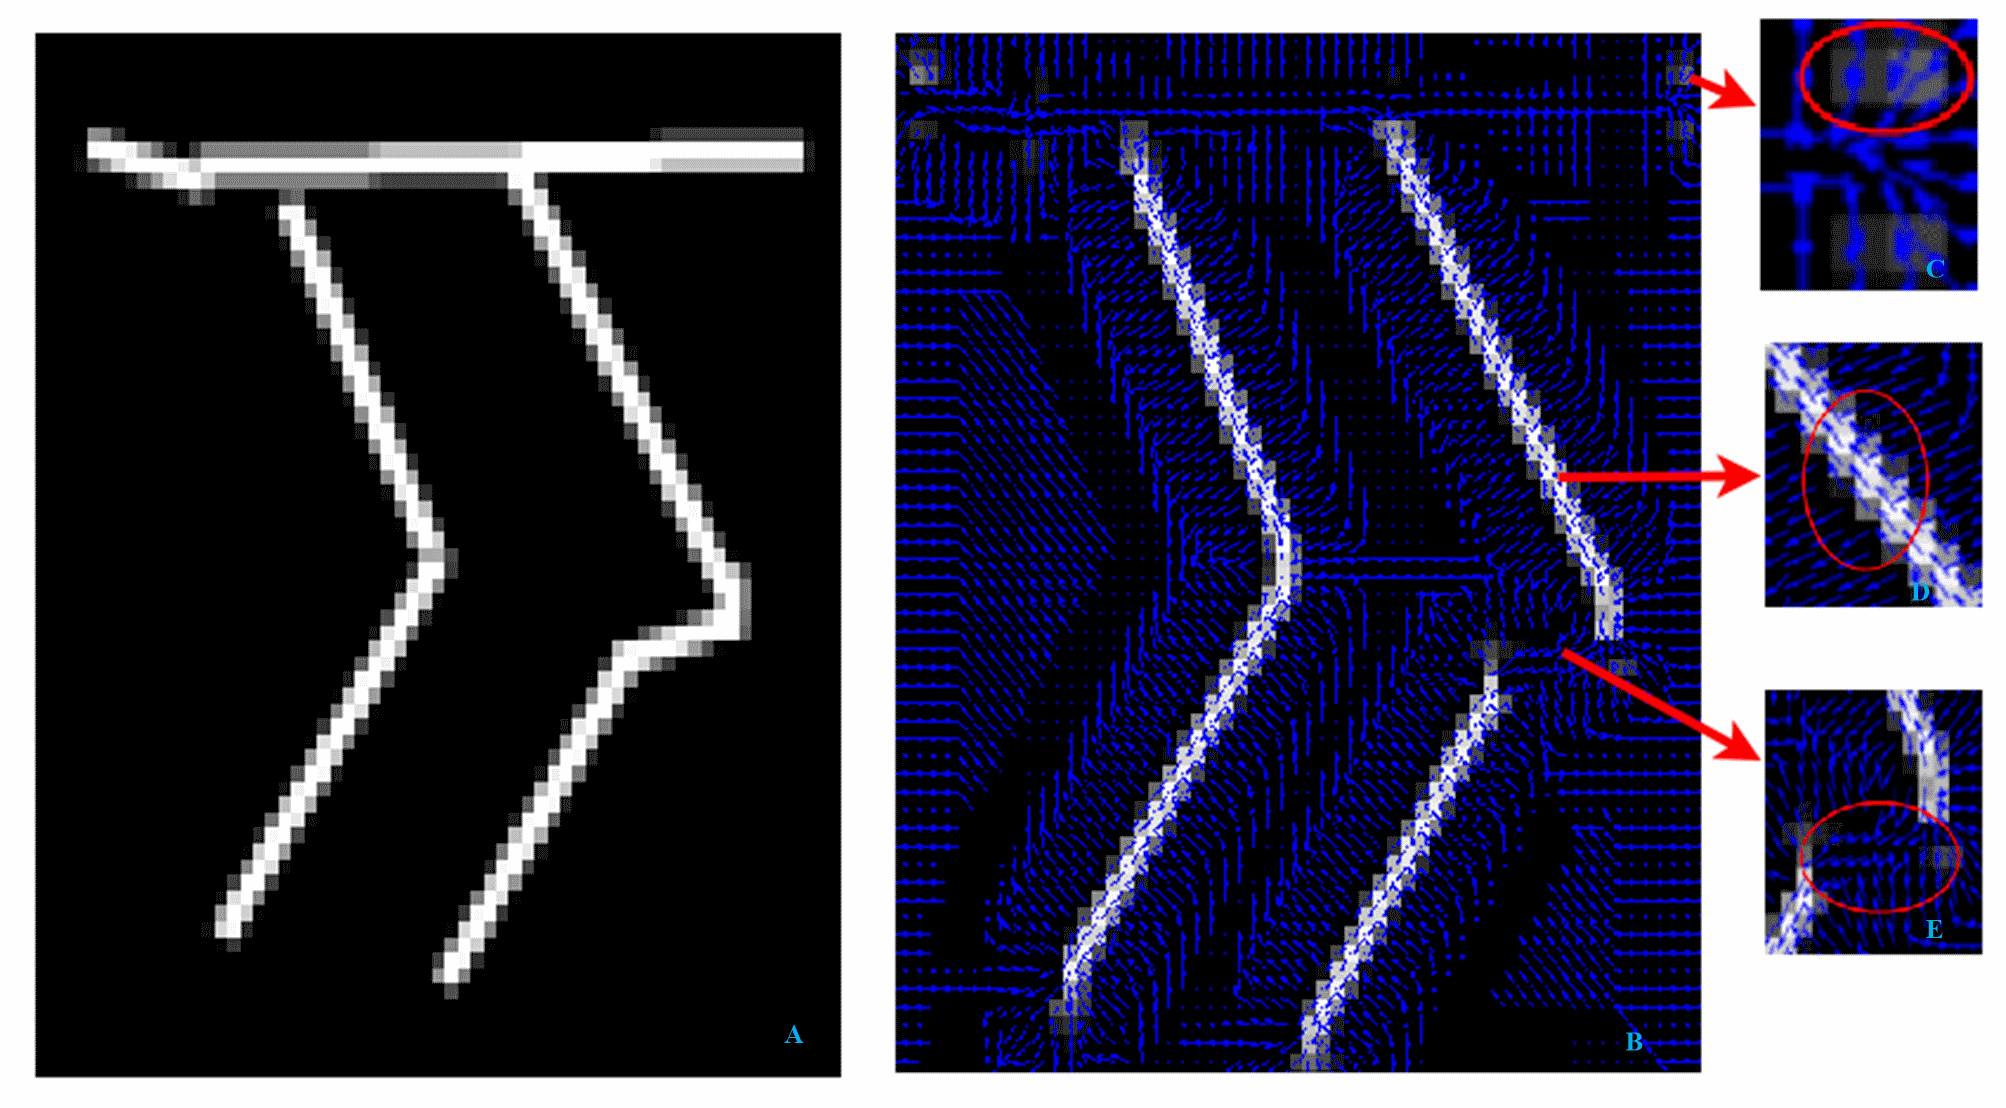
\includegraphics[scale=0.25]{figure/highResponse.png}
  \end{center}
  \caption[ISV principal direction estimation]{Figure \ref{responseAnalysis}A is used in place of original image to depict the structure similar to of ISV. \ref{responseAnalysis}A shows the response of maximum eigenvalue corresponding to scale = 1 for principal direction. In top right fig. \ref{responseAnalysis}C, shows few isolated regions from DLAV. These regions are outliers and will be removed. Figure \ref{responseAnalysis}D perfectly captures the response corresponding to principal direction. Figure \ref{responseAnalysis}E shows the region whose principal direction is lies outside the $[\alpha, \beta]$, hence no response is generated. These regions are merged.}
  \label{responseAnalysis}
\end{figure}

Some ISV might appear disconnected, or some isolated response from DLAV region might be outliers as shown in fig. \ref{responseAnalysis}C. This happens when region along center of ISV, appears parallel to x-axis i.e. the angle of principal direction with horizontal axis does not fall in $[\alpha, \beta]$ as depicted in fig. \ref{responseAnalysis}E. We connect the disjoint ISV's and remove outlier from DLAV based on the feature set extracted form each ISV region. 

The broken ISV when region along center of ISV, appears parallel to x-axis i.e. the angle of principal direction with horizontal axis does not fall in $[\alpha, \beta]$ as depicted in fig. \ref{responseAnalysis}E. Here we use morphological operation to link the broken vessels segmented. We compute the maximum response from all vessels using \eqref{eq:isv}. We binarize $r_{a}(x)$ based on value from Adaptive Niblack thresholding and call it $b_{r_a}$. Parameter k is the value of the scale (sigma) with the maximum eigenvalue from \eqref{eq:all}.

\begin{equation}\label{eq:all}
r_{a}(x) = \max_{\sigma} \lambda_{1}(x,\sigma) 
\end{equation}

At each potential vessel pixel from $b_{r}$, we apply morphological closing using linear structure. The direction of the linear structure is perpendicular to the x-axis direction. We set the length of the linear structure as 10 pixels in the experiments. We retain all those potential vessel pixel from $b_{r}$ that belongs to $b_{r_a}$.

\subsection{Post Processing}

There are some isolated response from DLAV region which are outliers as shown in fig. \ref{responseAnalysis}C. We follow similar approach as for linking vessels, but instead we work with maximum response from vessels from DLAV region \eqref{eq:dlav}. We binarize $r_{d}(x)$ based on value from Niblack thresholding and call it $b_{r_d}$. Parameter k is the value of the scale(sigma) with the maximum eigenvalue from \eqref{eq:dlav}.

\begin{equation}\label{eq:dlav}
r_{d}(x) = \begin{cases} \max_{\sigma} \lambda_{1}(x,\sigma) &\mbox{if } \alpha < \ h(x, \sigma) > \beta\\ 
0 & \mbox{if } otherwise \end{cases} 
\end{equation}

At each potential vessel pixel from $b_{r_d}$, we apply morphological closing using linear structure. The direction of the linear structure is parallel to the x-axis direction. We set the length of the linear structure as 10 pixels in the experiments. We remove all those potential vessel pixel from $b_{r}$ that belongs to $b_{r_d}$.


\section{Caudal Vein Plexus Segmentation}

After extracting ROI enclosing CVP as shown in fig. \ref{region}d. We use structural properties of CVP for segmentation. 

\begin{figure}[htb] \centering
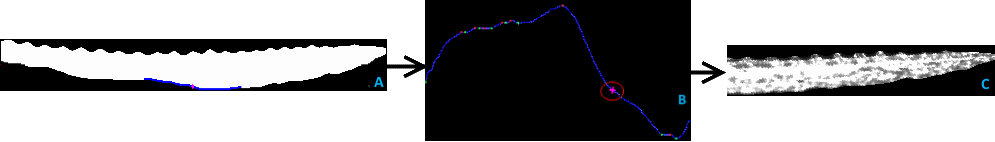
\includegraphics[scale = 0.55]{figure/cvpSeg.png}
	 \caption[CVP Segmentation]{Procedure for CVP segmentation. Figure \ref{seg}A is a region enclosing CVP. Curve $C$ in blue represents lower boundary of tail region along midpoint of tail. Figure \ref{seg}B $C$ is smoothed using moving average filter. Pink points represents local maxima and green points represents local minima. Circled point represents the CVP region start location. CVP start position is the mid point of the local curve with largest steepness. Figure \ref{seg}C is the segmented CVP obtained by masking out segmented region from fig. \ref{noiseRem}A with fig. \ref{seg}A from start location of CVP.}
 \label{seg}
\end{figure}

The intuition behind our method is that there is a high gradient associated with transition of PCV region to CVP region in zebrafish. For this purpose, we trace the curve $C$ along mid point $m$ of lower boundary of the tail.Lets $C$  be represented as:

					 \begin{equation}
						C =  ((x_{i}, y_{i}), i= 1,2,\ldots, n)						
						\end{equation} 
						
We compute the slope of the cure as: 

				\begin{equation}
				S =  (\frac{dy_{i}}{dx_{i}}, i= 1,2,\ldots, n)
				\end{equation} 
				
S is smoothed using moving average filter. Let H and L denote the set of local maxima and local minima along S. Let v = $(h_{i0}, l_{j0})$ denote local maxima and local minima, respectively, such that:

					  \begin{align*}
						\bmod(h_{i0} - l_{j0}) \geq \bmod(h_{i} - l_{j}), 
						    \forall h_{i} \in H, \forall l_{j} \in L,  j-1 \leq i \leq j
						\end{align*}  
						
Point $p$ where the CVP starts is given by:

				\begin{equation}\label{eq:cvp}
				p = \begin{cases} \frac{h_{i0} + l_{j0}}{2} & \mbox{if } H \neq \emptyset, L \neq \emptyset\\ 
				m &  otherwise \end{cases} 
				\end{equation}  
				\normalsize
				
$p$ signifies the mid point along the curve with maximum change in slope. CVP is obtained by masking region shown in fig. \ref{noiseRem}A from segmented region shown in fig. \ref{seg}C from start location $p$ of CVP.
\chapter{Feature Extraction}\label{chap:feature}
A toxicology screening can be observed as a typical two-class classification problem, consisting of feature extraction and classification process. In this chapter we will explain feature extraction algorithm for ISV and CVP.

\section{Intersegmental Vessel Feature Extraction}
ISV features are defined in terms ISV count; an average distance between ISV, total area of ISV; and an average ISV length. All terms were defined in pixels. Previous research have shown the quantification terms used in this work can use to analyze toxicity effect in ISV \cite{Feng05}, \cite{Tran07}, \cite{Vogt09}.

\begin{figure}[H]
  \begin{center}
    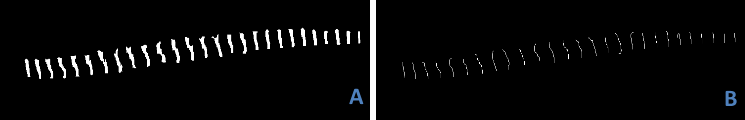
\includegraphics[scale=0.7]{figure/skeleton.png}
  \end{center}
  \caption[ISV skeleton]{Skeleton of ISV, used for calculating length of ISV.} 
  \label{skeleton}
\end{figure}

Our quantification procedure consists of reporting features: ISV count; average distance between ISV; total area of ISV; and average ISV length. We calculate these features for each of embryo. Features are obtained by performing connected component analysis. Number of connected component corresponds to ISV count. ISV distance is computed as the average of euclidean distance between ISV centroid, and the centroid of two adjacent neighboring ISV. Total area occupied by all components is ISV area. ISV length is computed by analyzing the skeleton of each of connected component. Image skeleton is obtained by thinning procedure explained in \cite{Lee94}.The general idea is to erode the ISVs surface iteratively until only the skeleton remains. The structure obtained is shown in fig. \ref{skeleton}(b). We decompose each individual vessel segments as individual graph for calculating ISV length. We perform graph analysis on each vessel and compute end points (pixels with less than 2 neighbors). For calculating the length of ISV we find the number of pixels connecting the end points. Average ISV length is computed by averaging over all graphs. Feature vector is formed by concatenating ISV count; average distance between ISV; total area of ISV; and average ISV length. 

\section{Caudal Vein Plexus Feature Extraction}\label{sec:cvp}
The study of the zebrafish CVP and its utilization as a model for screening assay has not been as prevalent as the ISV, and very few studies have attempted to identify regulators of CVP development. Previous research has primarily focused on using color, texture \cite{Tran07} and morphological changes \cite{Feng05} for toxicity analysis. Shape information, however, can be another attribute that can be evaluated. A shape descriptor can capture the outline of the shape that other color or texture-based descriptors may not be able to capture. Hence by quantification of the shape of CVP, and comparing it against that of a healthy embryo, we can identify changes in CVP due to exposure to toxins. This section will discuss utilization of gray level co-occurrence matrix (GLCM), histogram of oriented gradients (HOG), co-occurrence of histogram of oriented gradients gradient (Co-HOG) and weighted co-occurrence histogram of oriented gradients (gCo-HOG) for shape modeling.


\subsection{Gray Level Co-occurrence Matrix}

GLCM is a very well known texture analysis method \cite{haralick1973}, \cite{haralock1991}.  GLCM represents the angular and spatial over an image sub region. GLCM entries represents an estimate of the probability that two pixels with a specified displacement, d, and an angle, $\theta$ occurs in an image.  Statistical measures are derived from the co-occurrence matrix. The features we used include: energy, homogeneity, correlation, and contrast. For varying choices of d and $\theta$, we obtain a separate GLCM. The GLCM is implemented with certain degree of rotation invariance, which is achieved by combining the results from various angles. Angles 0, 45, 90, 135 are considered as effective choices. We analyzed results with varying value of k and obtained best performance with 9 pixel displacement. The results is combined by averaging the GLCM for each angle and concatenating energy, homogeneity, correlation, and contrast into one feature vector.

\subsection{Histogram of Oriented Gradients}

HOG descriptor first proposed by Dalal and Triggs \cite{Dalal05} has been used in many different problems in computer vision, such as pedestrian detection \cite{Wada09}, face recognition \cite{Deniz11}, object recognition \cite{Bosch07} and text recognition \cite{Wang10}. HOG features are extracted from image by first computing gradient orientation at every pixel. Orientations of gradients are quantized into histogram bins and each bin has an orientation range. Image is divided into blocks and in each block a histogram of oriented gradients is computed. HOG feature consists of concatenation of histogram of oriented gradients over all blocks. 

\begin{figure}[htb] 
 \centering
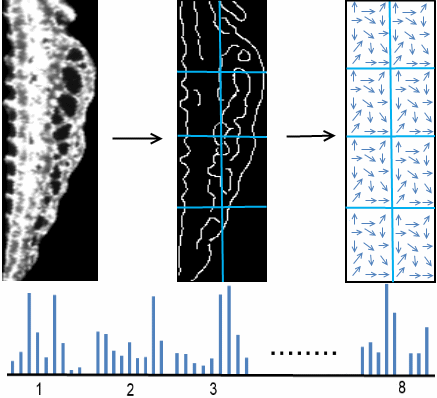
\includegraphics[scale=0.75]{figure/hog.png}
  \caption[HOG features from a CV image]{Extraction of HOG features from a CV image. (left) Original image. (center) Edge contours are extracted using an edge detector, image is divided into 8 blocks. (right) HOG vector is extracted from each sub region. (bottom) Concatenation of all the HOG vectors to obtain the HOG features for image.}
 \label{hog}
\end{figure}

In our case, HOG are computed on edge contours extracted using the canny edge detector (fig. \ref{hog}(center)). The gradients are computed using a Sobel mask. The HOG descriptor is quantized into $K$ orientation bins, each over an orientation range. The weight from each contour point depends on its gradient magnitude and is added to its orientation bin. Each bin in the histogram represents the sum of gradient magnitudes that have orientations within a certain angular range. 

HOG are invariant to 2d rotation and illumination variations. On the other hand, HOG captures orientation of only isolated pixels, ignoring spatial relationship among neighboring pixels. Co-HOG captures spatial information and is more powerful in describing local structure. With spatial structure, more shape information of object can be captured.

\subsection{Co-occurrence of Histogram of Oriented Gradients}\label{sssec:cohog}

Co-HOG is an extension of HOG. Co-HOG captures spatial information by measuring probability of oriented gradients between pairs of pixel. A pixel pair can be represented by an offset $(x, y)$, which captures the spatial relationship of the two points. As shown in fig. \ref{cohog}(left), we define 31 offsets including zero offset for a given point. The black pixel in the center is the pixel under consideration and the neighboring blue pixels are with different offsets. Each neighboring pixel in blue color forms an orientation pair with the center black pixel and accordingly votes to the co-occurrence matrix. For each pixel in the image of size $M \times N$, the orientations ranging between $[0, 360]$ are quantized into eight orientation bins. Co-occurrence matrix at a specific offset $(x, y)$ is defined as:
		
			\begin{equation}\label{eq:cohog}
				C_{x,y}(i, j) = \sum_{p}\sum_{q}\begin{cases} 1, & \mbox{if } I(p, q) = i, I(p + x, q + y) = j\\ 
				0, &  otherwise \end{cases} 
				\end{equation} 
				\normalsize 
				
The Co-HOG descriptor is formed by concatenation of components of the co-occurrence matrix of each offset including offset 0. Co-HOG obtains 31 co-occurrence matrices. There are $8 \times 8 = 64$ elements in the co-occurrence matrix (fig \ref{cohog}(right)). The co-occurrence matrix calculated with zero offset has only 8 values.

%There are $8 \times 8 = 64$ elements in the co-occurrence matrix (fig \ref{cohog}(right)). The co-occurrence matrix calculated with zero offset has only 8 values. 8 rectangular regions are tiled $M/4 \times N/2$ with no overlap. More tiles are made along the image width as CV occupies more region along width as compared to height. Finally, co-occurrence matrices from all the rectangular regions are concatenated into one vector. Thus the dimension of our feature is $(64 \times 30 + 8) \times 8 = 15424$. 
Co-HOG extracts both local and global shape information, with varying offset sizes. 

One potential limitation of co-occurrence histograms of oriented gradients is that both strong and weak gradients provide the same contribution in representing the spatial structure.  To address this limitation, we investigate the inclusion of gradient strength in the generation of the histogram.

\begin{figure}[htb] 
 \centering
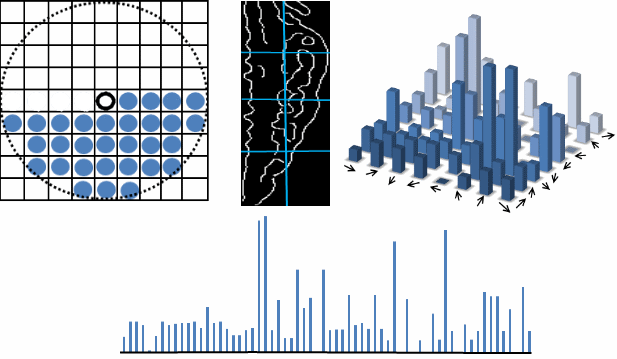
\includegraphics[scale=0.75]{figure/cohog.png}
  \caption[Co-HOG features from a CV image]{ Extraction of Co-HOG features from a CV image. (left) Pixel offset. (center) Edge contours are extracted using an edge detector, image is divided into 8 blocks. (right) Co-HOG vector is extracted from one region. (bottom) concatenation of all the Co-HOG vectors to obtain the Co-HOG features for image.}
 \label{cohog}
\end{figure}

As shown in \cite{Pang12}, we treat gradient as forces and use vector addition to combine forces using:
	
				\begin{equation}\label{eq:add}
				C_{x,y} = C_{x,y} + \|g_{1} + g_{2}\| 
				\end{equation}
				\normalsize 
				
where $C$ is the co-occurrence matrix at a specific offset $(x, y)$ as defined in equation \ref{eq:cohog}, $g_{1}$ is the gradient magnitude at location $(p, q)$, and $g_{2}$ is the gradient magnitude at location $(p + x, q + y)$. The gCo-HOG feature descriptor of the whole image can then be constructed by concatenating all the regions features. The gCo-HOG is normalized to sum to unity.

\section{Vasculature Time-lapse Features} \label{sec:timelapse}

There are various challenges associated with live imaging oz zebrafish. One such complication is, zebrafish embryos twitch, so that growth and motion of embryos are not uniform across the 3D field. Imaging captures the dynamics of blood vessel formation over time. In order to quantify these morphological changes, i.e. how much vascular structure has changed over a period of time, it is necessary to compensate for any movements caused by the growing embryo. Thus, in order to record the temporal changes occurring due to vessel growth, it is necessary to establish spatial correspondence between blood vessels that may appear displaced due to embryo movement. Thus quantification of temporal vascular growth can be seen as a problem of image registration. we use a non-rigid registration approach to align images. Non-rigid mapping is based on complete correspondence of images and includes a deformation model as the underlying transformation. We utilize free-form deformation based on B-splines for growth monitoring, and use intensity differences as a similarity measure.  

\subsection{Vasculature Registration}
The goal of image registration is to find an optimum mapping that aligns two images. Since deformations are important for quantification of changes in images, it is necessary to find a mapping between two time points as accurately as possible. In our case we need to quantify blood vessel growth independent of motion artifacts.  Hence we need a registration approach that establishes vessel correspondence between successive time frames. Affine and rigid registration approaches are mainly based on local stretching of images, and hence do not adequately capture structural changes.

Many applications in medicine require that object is modified in global scale. Therefore, we have used free-form deformation (FFD). Free form deformation deforms an object by warping the image geometry in which the object is localized. The nature of deformation varies widely across different time points; hence it is difficult to use traditional B-spline registration, which is based on many parameters. If we only select few parameters, an approximate match can be obtained, whereas many parameters incur added computational costs. Hence, we have used FFD based on hierarchical B-splines for multilevel nonlinear registration \cite{Lee97}. The underlying idea of FFD is based on deforming an object by manipulating a mesh of 2D points.

Let $\Omega  = \left\{(x,y)\mid 0 \leq\ x \geq X, 0 \leq\ y \geq Y \right\}$ be the domain of $2d$ points. Let $\Omega$ denote a $n_{x}\times n_{y}$ mesh of control points with uniform spacing $\Delta$. Let $\Omega_{ij}$ be the value of ij-th control point located at $(i,j)$. The FFD f can be written as:

\begin{equation}
f(x,y) = \sum_{m=0}^{3}\sum_{l=0}^{3}B_{l}(s)B_{m}(t)\Omega_{i+l,j+m}
\end{equation}	

where, 
$i = \floor*{\frac{x}{n_{x}}} - 1$ 
$j = \floor*{\frac{y}{n_{y}}} - 1$ ,
$s = \frac{x}{n_{x}} - \floor*{\frac{x}{n_{x}}}$,
$t = \frac{y}{n_{y}} - \floor*{\frac{y}{n_{y}}}$.
$B_{l}$ and $B_{m}$ are uniform cubic B-spline basis function defined as:

\begin{equation}
B_{0}(s)=  \frac{(1-s)^{3}}{6}
\end{equation}	
\begin{equation}
B_{1}(s)=  \frac{(3s^{3}-6s^{2}+4)^{3}}{6}
\end{equation}	
\begin{equation}
B_{2}(s)=  \frac{(-3s^{3}-3s^{2}+3s+1)^{3}}{6}
\end{equation}	
\begin{equation}
B_{3}(s)=  \frac{s^{3}}{6}
\end{equation}	

They weigh the contribution of each control point to $f(x,y)$ based on its distance to $(x,y)$. The problem of deriving function f is reduced to solving for the control points in $\Omega$. The control points in $\Omega$ behave as parameters for transformation. The degree of non-rigid deformation depends highly on the size of control points. Dense mesh can increase number of degrees of freedom, hence providing more flexibility and consequently an increase in computational complexity. In order to achieve the tradeoff between degree of freedom and computational complexity, we use a hierarchical multiresolution \cite{Lee97} approach, in which the resolution of the control mesh is increased, along with the resolution of image in an iterative loop. Consider a hierarchy of control mesh $\Omega_{0}, \Omega_{1},\ldots,\Omega_{h}$ overlaid on domain $\Omega$. For simplicity, we will assume decreasing space as we move from $\Omega_{s}$ to $\Omega_{s+1}$. Similar to above, we will have FFD $f_{s}(x,y)$ for each control mesh. Their sum defines the overall transformation model.

\begin{equation}
f(x,y)= \sum_{s=1}f_{s}(x,y)
\end{equation}
Calculation of FFD for each control lattice introduces a significant overhead. To avoid this overhead, B-spline refinement can be applied hierarchically to control mesh. This can be achieved by B-spline subdivision algorithm. In this case, the control point mesh at level s is generated by using the mesh control points from level $s-1$. More details can be found in \cite{Forsey88}. To achieve correspondence between two images acquired at different time points, we have used a similarity criterion based on sum of squared difference (SSD):

\begin{equation}
SSD = \frac{1}{n} \sqrt{(\sum{(I(t_{0})-T(I(t)))^{2}}}
\end{equation}

\subsection{Vasculature Morphology}\label{quantification}

Blood vessel growth is quantified by recording the temporal occurrence of differences in pixel intensities along registered vascular structures. Registration is performed on pair of consecutive images $(I_{t},I_{t+1})$. $I_{t}$ is warped to $I_{t+1}$ to give $I_{reg_t}$. Measuring the difference (pixel changed) between $I_{t+1}$ and $I_{reg_t}$  provides a standard for change quantification. This protocol is shown in fig. \ref{reg}

\begin{figure}[htb] 
 \begin{center}
    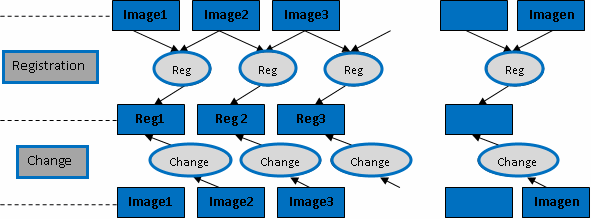
\includegraphics[scale=0.75]{figure/reg_overview.png}
  \end{center}
  \caption[Quantification Procedure]{For a given sequence of images, image i is registered to (i + 1). Measuring the difference between registered images i and (i + 1), provides the change in number of pixels.}
  \label{reg}
\end{figure}

, where $\Delta_{t}$  is the change in number of pixels at time t.
\begin{equation}
\Delta_{t}= I_{t+1} - I_{reg_t}
\end{equation} 


The change measured over the entire imaging cycle can be characterized by the function $f(\Delta_{t})$ given by:
\begin{equation}
f(\Delta_{t})= \left\{\delta_{t}\right\}_{t=1}^{m}
\end{equation}

In next chapter, we will give details corresponding to zebrafish data used for experiments.
\chapter{Materials}\label{chap:materials}

%We have worked on two types of dataset. For, first data we have 2d images of fully developed zebrafish, showing complete anatomy. For, this data we have presented segmentation and quantification methodology. Second data consist of 3d temporal data of zebrafish vasculature. For, this we presented a technique for temporal vasculature growth. 

Zebrafish embryo images are collected at Center for Nuclear Receptors and Cell Signaling, Department of Biology and Biochemistry, University of Houston. Zebrafish (Danio rerio) are reared and maintained at $28.5^{\circ}$ C as previously described \cite{westerfield00}, and in accordance to the standard operating protocols approved by the Institutional Animal Care and Use Committee at University of Houston. A stable line of Tg(kdrl:EGFP)$mitfa^{b692}$ is generated by crossing Tg(kdrl:EGFP) with $mitfab^{692/b692}$ (Zebrafish International Resource Center, Eugene, OR) to facilitate GFP visualization without obstruction from melanophores. Embryos are collected from natural mating and staged accordingly \cite{Kimmel95}.

Two dimensional data is acquired for ISV and CVP analysis. Three dimensional time lapse data is acquired to study overall growth in vasculature of zebrafish. 

\section{Two Dimensional Data}
Zebrafish embryos are treated with chemicals selected from phase I of ToxCast chemical library (http://www.epa.gov/ncct/toxcast/chemicals.html) and solubilized in dimethyl sulfoxide (DMSO).

\subsection{Chemical Treatments}
Tg(kdrl:EGFP) $mitfa^{b692}$ embryos are harvested in a petri dish after mating. At approximately 3 hpf, embryos are sorted and placed in 6-well plates (n = 20), followed by a single chemical treatment without renewal at 100 nM, 250 nM, 500 nM, 1 $\mu$ M, 10 $\mu$ M and 20 $\mu$ M, unless otherwise noted. Working dilution stocks of all chemicals are made such that the final concentration of the vehicle DMSO is at 0.1\%. Each well contained a final volume of 3 mL of embryo medium, E3 (5 mM NaCl, 0.17 mM KCl, 0.33 mM CaCl2, 0.33 mM MgSO4). Control embryos are treated with 0.1\% DMSO. The embryos are incubated at $28.5^{\circ}$ C until 72 hpf, during which they are assessed for vascular perturbations. 

\subsection{Imaging}
At 72 hpf, control and treated embryos are manually dechorionated, if necessary, and anesthetized with 0.04\% MS-222 (Pentair Aquatic Eco-Systems, Apopka, FL). Embryos are manually oriented and imaged using a 4X objective on an Olympus IX51 fluorescence microscope equipped with an Olympus XM10 camera and cellSens Dimension software (Olympus, Center Valley, PA).

\begin{figure}[htb] 
 \begin{center}
    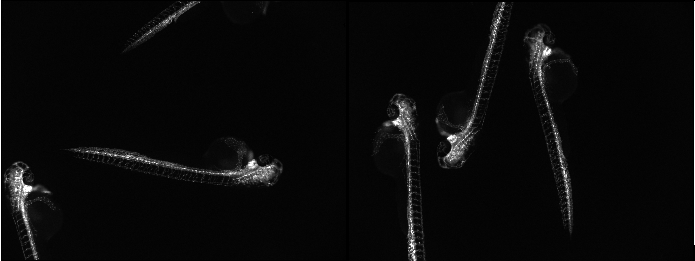
\includegraphics[scale=0.75]{figure/fishData.png}
  \end{center}
  \caption[Zebrafish full anatomy 2d dataset]{Original 2d images of zebrafish capturing zebrafish full anatomy.}
 \label{2dFish}
\end{figure}


\section{Three Dimensional Time - Lapse Data}

Zebrafish embryos are treated with Sodium (meta) arsenite (NaAsO$_{2}$) with 400 $\mu$g dosage. 

\subsection{Chemical Treatment}
Sodium (meta)arsenite (NaAsO$_{2}$) is purchased from Sigma-Aldrich (St. Louis, MO) and dissolved in ultra pure deionized water(vehicle). Tg(kdrl:EGFP)$mitfa^{b692}$ embryos are harvested in a petridish after mating. Then, they are sorted and placed in 6-wellplates (N = 10-30) in 3 mL of embryo medium, E3 (5 mM NaCl,0.17 mM KCl, 0.33 mM CaCl$_{2}$, 0.33 mM MgSo$^{4}$), followed by arsenite treatment at 400 $\mu$g/L (3.08 mM) without renewal. The embryos are incubated at $28.5^{\circ}$C until 72 hpf, at which they are manually dechorionated, if necessary, and assessed for vascular perturbation and other developmental malformations. For determining the window of effect, embryos are treated with arsenite at 400 $\mu$g/Lat 0-24 hpf, 24-48 hpf, or 48-72 hpf. After exposure time is complete, embryos are washed multiple times and allowed to continue to develop in E3 at $28.5^{\circ }$C until assessment at 72 hpf.For RT-qPCR, 30 embryos are pooled as one biological sample in 3 mL of E3 and treated with arsenite at 10 $\mu$g/L, 50 $\mu$g/L, 100 $\mu$g/L, 200 $\mu$g/L, or 400 $\mu$g/L up to 72 hpf. To examine RNA levels at different time points via RT-qPCR, embryos are treated with arsenite at 400 mg/L up to 18 hpf, 20 hpf, 24 hpf, 28 hpf, or 48 hpf. Control embryos are treated with vehicle.


\subsection{Imaging}

72 hpf control and arsenite-treated Tg(kdrl:EGFP)$mitfa^{b692}$ embryos are manually dechorionated, if necessary, and anesthetized with 0.04\% MS-222 (Pentair Aquatic Eco-systems, Apopka, FL). Embryos are then manually oriented and mounted in 0.8\%low-melt agarose (LMA; Sigma), and imaged using an Olympus Fluoview 1000 confocal fluorescence microscope with a 4X or 20X objective and 50 or 30 z-plane optical slices, respectively. Images are then rendered by Olympus Fluoview software and projection are generated using ImageJ. Brightfield images are captured with a Nikon DS-Fi1 color camera attached to a Nikon AZ100M microscope with a 4X objective and 25 z-plane optical slices, and then rendered by Nikon NIS-Elements software.2.7. 

\subsection{Time-lapse imaging}

Tg(kdrl:EGFP)$mitfa^{b692}$ embryos are treated with arsenite, as described above. At approximately 18 hpf, control and treatede mbryos are manually dechorionated, anesthetized with 0.04\%MS-222 and mounted in 0.3\% LMA on MatTek glass bottom dishes (MatTek Corporation, Ashland, MA). The 0.3\% LMA mounting media is supplemented with 0.04\% MS-222 and arsenite at concentrations matching to that of the exposure solutions. E3 with MS-222and arsenite is added following LMA solidification and the dishes are sealed with parafilm. 100 z-plane optical slices are acquiredon an Olympus Fluoview 1000 confocal fluorescence microscope over a span of 15 h with 15 min time intervals. Images are then processed by Olympus Fluoview software and projections are animated into a time-lapse movie using ImageJ.

\begin{figure}[htb] 
 \begin{center}
    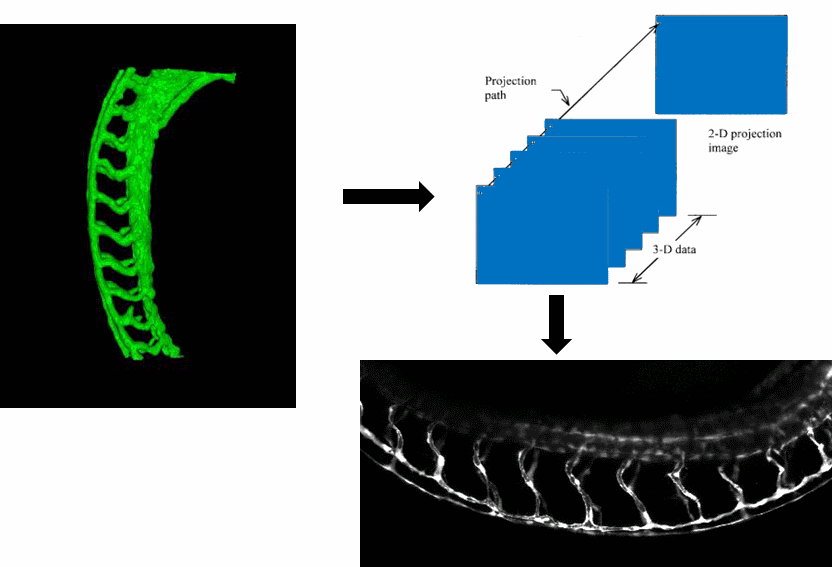
\includegraphics[scale=0.5]{figure/projection.png}
  \end{center}
  \caption[Maximum intensity projection]{Maximum intensity projection is computed by selecting the brightest voxel along z-axis.}
 \label{mip}
\end{figure}

\begin{figure}[htb] 
 \begin{center}
    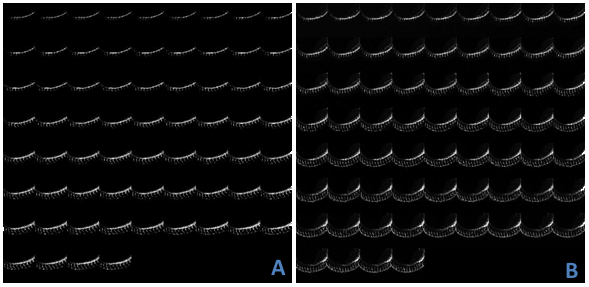
\includegraphics[scale=0.75]{figure/mon.png}
  \end{center}
  \caption[Zebrafish vasculature dataset]{(A) Vascular development for unexposed embryo. (B) Vascular development for arsenic exposed embryo.}
 \label{2dVascular}
\end{figure}

Images are generated in TIFF format with 8-bit intensity depth. Image size is 512 pixels by 512 pixels and 640 pixels by 480 pixels. Maximum Intensity projection (MIP) (fig. \ref{mip}) is computed for stack of images. MIP algorithm selects the brightest voxel along the z-axis and projects it on the orthogonal image plane. Figure \ref{2dVascular} shows MIPs for unexposed and exposed embryo.
\chapter{Zebrafish Analysis}\label{chap:results}

This chapter is divided into three sections. First section presents result related to ISV analysis. We will compare proposed automated segmentation of ISV against manual segmentation. Further to identify whether chemicals from ToxCast Phase I library are vascular disruptor compounds, we present how ISV features can be used to discriminate healthy embryo from abnromal embryos. ISV features are used to train a linear classifier for depicting embryos impacted with toxicity. 

Second section will focus on CVP analysis, presenting classification results using GLCM, HOG, Co-HOG, and proposed gCo-HOG. In third section, we will explore the relationship between increasing dosage of chemicals with impact on ISV, and CVP separately. We will discuss how many chemicals impacted ISV and CVP or both.

Last section will present results showing variations in temporal growth of embryo for healthy against treated. 


\section{Intersegmental Vessel Analysis}\label{sec:isvanalysis}
ISV results are presented for entire zebrafish vasculature recorded from the fluorescence microscope. 

\subsection{Segmentation Analysis}
Segmentation of ISV can be a time consuming process. ISVs occur in various size and shows huge variation in intensity. Method in section \ref{sec:isvseg} to segment the ISV from zebrafish images. The accuracy of the automatic segmentation of ISVs is determined by the comparisons between manual segmentation and the automated. 30 randomly chosen ISVs are manually segmented in the RGB color space, and compared. Vessels are visually inspected by two users (fig. \ref{isvseg}). 


Accuracy, Precision and recall measures and F-score are used to define error \cite{Martin01}. The error measures used are defined as follows:
\begin{equation}
Accuracy = \frac{tp + tn}{(tp + tn + fp + fn)}
\end{equation}

\begin{equation}
Precision = \frac{tp}{(tp + fp)}
\end{equation}

\begin{equation}
Recall = \frac{tp}{(tp + fn)}
\end{equation}

\begin{equation}
F - score = 2*\frac{(Precision * Recall)}{(Precision + Recall)}
\end{equation}

 \begin{figure}[H] 
 \begin{center}
    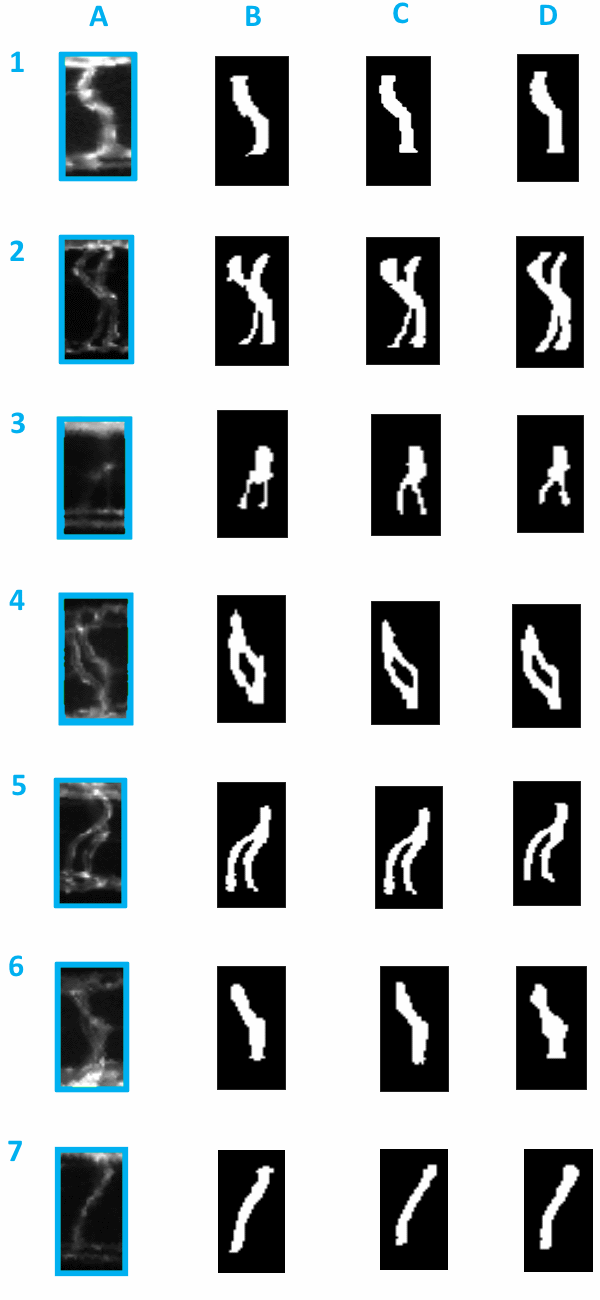
\includegraphics[scale=0.5]{figure/isvSegmentation.png}
  \end{center}
  \caption[ISV segmented images]{Comparison between automated segmentation and manual segmentation by user1 and user 2 of zebrafish embryos. (A) Analyzed ISV (B) Automated segmentation (C) User 1 segmentation (D) User 2 segmentation}
 \label{isvseg}
\end{figure}


where tp is the number of true positives, tn is the true negatives count, fp is the number of false positives and fn is the number of false negatives. The output of the segmentation is a binary vector with the same size as the image. A true positive is when output of
our segmentation is 1 when manual users marked it as 1, a true negative is when the output of the segmentation is 0 while the manual users labeled it as 0, a false positive is when the output of the segmentation is 1 when users label is 0, and a false negative is when the output of the segmentation is 0 while the users label is 1. We used the above mentioned error to quantitate how close the automated method is to manual segmentation. We have shown the results for 30 randomly chosen zebrafish ISVs by two users in fig. \ref{segResult}. 


\begin{table}[htb] 
\begin{center}
	\caption{Segmentation results for ISV} 
	
    \begin{tabular}{| c | c | c |}
    \hline\hline
    \textbf{Analysis} & \textbf{User 1}  & \textbf{User 2} \\ \hline \hline
		Precision & 0.847 & 0.839  \\ \hline
		Recall & 0.826 & 0.828  \\ \hline
		Accuracy & 0.952 & 0.951  \\ \hline
		F - score & 0.834 & 0.830  \\ \hline
    \end{tabular}
		\label{table:segRes} 
\end{center}
\end{table}

The average accuracy for the ISVs with manual users are $0.952$ and $0.951$. Average f-score for both users are 0.830 and 0.832. More detailed results are presented in table \ref{table:segRes}. These results indicate that the automated segmentation is comparable to that by manual segmentation. 


 \begin{figure}[H] \centering
 \begin{center}
    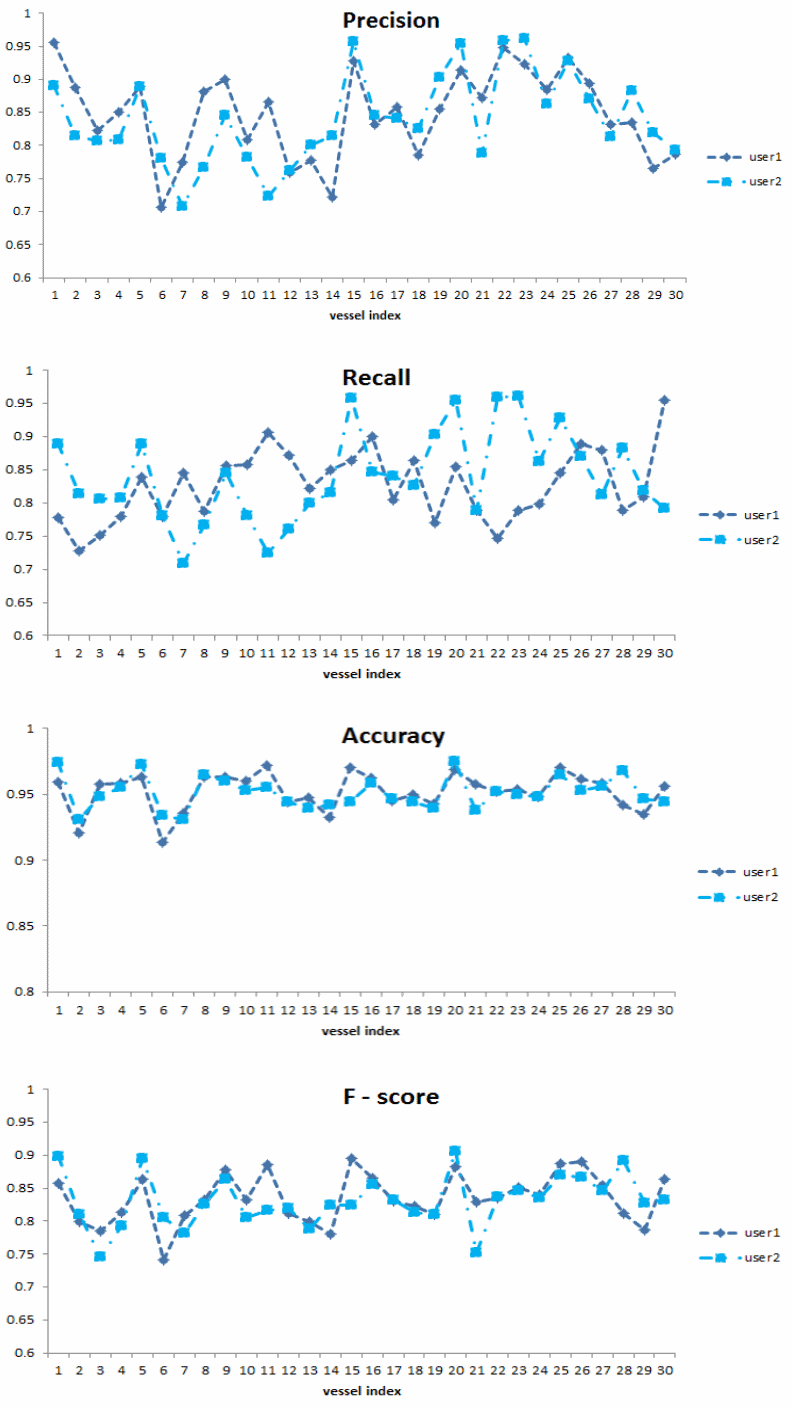
\includegraphics[scale=0.45]{figure/isvSegResult.png}
  \end{center}
  \caption[Comparison between the automated segmentation and manual segmentation of ISV.]{(a) Our approach have an average accuracy of 0.95 with user 1 and user 2. (b) Our approach have an average precision of 0.83 and 0.84 with with user 1 and user 2. (c) Average recall for both users is 0.83. (d) Lastly, average f - score for user are 0.83.}
 \label{segResult}
\end{figure}

\subsection{Toxicity impacts Intersegmental Vessels}

To identify whether chemicals from ToxCast Phase I library are vascular disruptor compounds (VDCs), 38 chemical are tested in a range of concentrations on zebrafish embryos from 3 hpf to 72 hpf in a single static exposure. Typically, the chemicals are tested from 100 nM to 20 $\mu$M. If the chemical exposures are lethal, lower and narrower dosages are tested. Visual analysis showed changes in ISV morphology due to chemical treatment. ISV abnormalities included the absence of ISV (fig. \ref{toxicity}), or thin and underdeveloped ISV (fig. \ref{toxicity}C). Quantitative image analysis is performed on the vascular disruption in the ISVs. 

\begin{figure}[H]\centering
  \begin{center}
    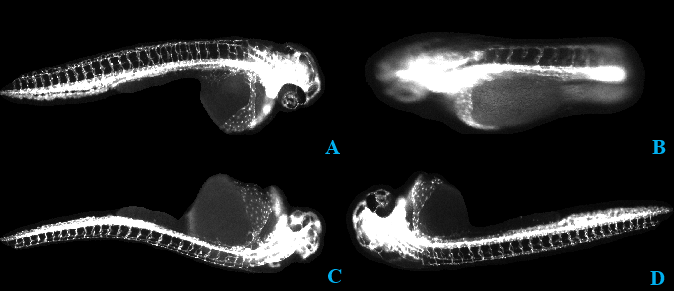
\includegraphics[scale=0.35]{figure/toxicityEffect.png}
  \end{center}
  \caption[Effect of toxins on ISV]{ Severity of toxins effect on zebrafish ISVs. High dosage can act as a ISV disruptor, and these effects can be quantified in terms of ISV count; average distance between ISV; total area of ISV; and an average ISV length. Figure \ref{toxicity}A shows an increment in ISV count, whereas \ref{toxicity}B shows decrement in ISV count.  Figure \ref{toxicity}C, \ref{toxicity}D embryos have small size ISV and occupy less area.}
  \label{toxicity}
\end{figure}


ISVs are first isolated from images using algorithm presented in section \ref{sec:isvseg} from the whole embryo and measured for ISV length, ISV distance, number of ISVs and ISV area. All terms are defined in pixels. We reported quantification results for 38 toxins. Previous research have shown the quantification terms used in this work can be used to analyze toxicity effect in ISV \cite{Feng05}, \cite{Tran07}, \cite{Vogt09}. Figure \ref{isvplots} shows with increasing toxins dosage, the ISV disruption becomes more prominent. Average ISV count, average distance between ISV, average ISV area and an average ISV length gradually decreases with increasing chemical dosage. %Details about an average ISV length, an average number of ISVs average ISV distance and an average ISV area are presented in table \ref{table:isvScreen}

To aid HTS of ISV for toxicity, we utilized features quantification to train a linear SVM classifier to identify zebrafish embryo with morphological changes. Dataset consists of 380 images of ISV. 190 images in the dataset did not show any abnormalities, while the remaining 190 images shows morphological changes to the ISV due to toxicity. Labels are visually obtained. We split the data into two parts. $1/3$ of data is used for parameter estimation for SVM and rest $2/3$ is used for training and testing. Parameters $(C, \gamma)$ are determined based on a grid-search that is conducted among $C$ $\epsilon$ ${2^{-10}, 2^{-4}, \cdots, 2^{10}}$ and $\gamma$ $\epsilon$ ${2^{-10}, 2^{-4}, \cdots, 2^{10}}$ with 3-fold cross-validation. Using the parameter values that achieved the best cross-validation accuracy, we then built a new model on the remaining data set, using 3-fold cross-validation. The optimal $C$ and $\gamma$ parameters are found to be 0.5 and 16, respectively, resulting in SVM model classification accuracy of $93.03\%$.

\begin{landscape}\centering
\begin{figure}[htb]
 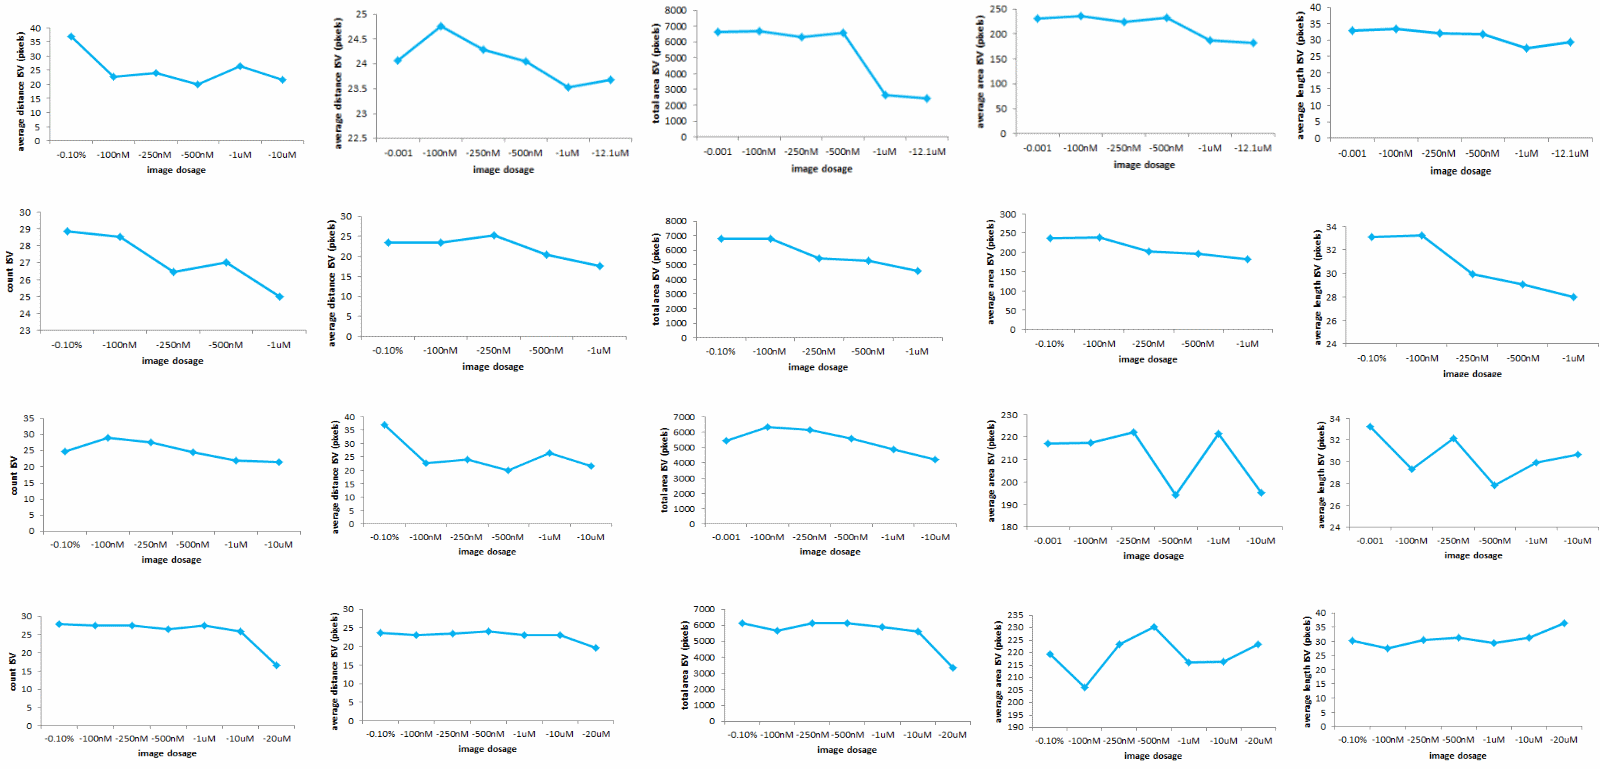
\includegraphics[scale=0.45]{figure/analysisPlot.png}
\caption[ Effect of toxins on ISV morphology]{Plots for various chemicals with variable dosage in comparison too untreated embryo (0.1\%). Each row corresponds to different chemicals. Within each row first plot shows variation in ISV count; Average ISV distance; Average ISV Area; Total SIV area;}\label{isvplots}
\end{figure}
\end{landscape}


\section{Toxicity impacts Caudal Vein Plexus}\label{sec:cvpanalysis}

CVP analysis results are presented for entire zebrafish vasculature recorded from the fluorescence microscope. We will present CVP analysis results using features explained in section \ref{sec:cvp}. We will empirically validate choice of parameters used for analysis. Dataset consists of 180 images of various size ($163 \times 55 - 331 \times 150$ pixels). 90 images in the dataset do not show any abnormalities, while the remaining 90 images show structural changes to the CVP due to toxicity effects (fig. \ref{cv} shows the images of healthy and treated zebrafish embryo). Labels are visually obtained. On similar lines ad CVP toxicity analysis We split the data into two parts. $1/3$ of data is used for parameter estimation and rest $2/3$ is used for training and testing. Parameters $(C, \gamma)$ are determined based on a grid-search that is conducted among $C$ $\epsilon$ {$2^{-10}, 2^{-4}, \cdot, 2^{10}$} and $\gamma$ $\epsilon$ {$2^{-10}, 2^{-4}, \cdot, 2^{10}$} with 3-fold cross-validation. Using the parameter values that achieved the best cross-validation accuracy, we then built a new model on the remaining data set, using 3-fold cross-validation. 

\begin{figure}[htb] \centering
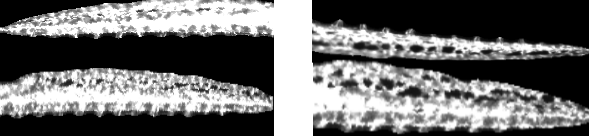
\includegraphics[scale=0.95]{figure/cv.png}
  \caption[Healthy and treated CVP]{Image on left shows healthy CVP and on right is the CVP observed for an embryo exposed to toxin. Loopy structure develops in CVP region for the treated embryo.}
 \label{cv}
\end{figure}

\subsection{Gray Level Co-occurrence Matrix Analysis}

Features energy, homogeneity, correlation, and contrast are calculated from each image using GLCM representing our image. We computed results with varying d ranging from 1-15. We obtain best results using d = 9. Table \ref{table:accglcm} shows comparison between accuracies with varying d. 

\begin{table}[h] 
\begin{center}
	\caption{Recognition results (\%) for GLCM with varying d} 
    \begin{tabular}{| c | c |}
    \hline
    \textbf{d} & \textbf{accuracy} \\  \hline \hline
		 1 & 73.02 \\  \hline
		 2 & 71.42 \\  \hline
		 3 & 80.15 \\  \hline
		 4 & 76.19 \\  \hline
		 5 & 76.91 \\  \hline
		 6 & 79.36\\  \hline
		 7 & 80.95 \\  \hline
		 8 & 76.98 \\  \hline
		 9 & 80.95 \\  \hline
		 11 & 75.39\\  \hline
		 12 & 80.74 \\  \hline
		 13 & 80.95 \\  \hline
		 14 & 78.57 \\  \hline
		 15 & 80.57 \\  \hline
    \end{tabular}
		\label{table:accglcm} 
\end{center}
\end{table}


The optimal $C$ and $\gamma$ parameters are found to be 65536 and 0.03, respectively, resulting in SVM model classification accuracy of $80.95\%$.

\subsection{Histogram of Gradient Analysis}
8 rectangular regions are tiled $M/4 \times N/2$ with no overlap. More tiles are made along the image width as CVP occupies more region along width as compared to height. To compare the effect of orientations, we generate histograms with orientation range from $[0, 360]$ and $[0, 180]$. Histograms with bin size $K$ ranging from 5 to 10 are evaluated. We got a best performance with bin size 6, 8, 9, 10 for $[0, 360]$ orientation (table \ref{table:acchog360} and \ref{table:acchog180}). We choose bin size of 6 and orientation range as $[0, 360]$. Thus the dimension of our feature is $(6 \times (4 \times 2)) = 1$. The optimal $C$ and $\gamma$ parameters are found to be 16 and 0.5, respectively.

\begin{table}[h] 
\begin{center}
	\caption{Recognition results (\%) for Co - HOG with varying bin size $K$ for $[0, 360]$ orientation} 
    \begin{tabular}{| c | c | c | c | c | c | c |}
    \hline
    \textbf{d} &  5  &  6  &  7  &  8  &  9  &  10\\  \hline
		 \textbf{accuracy} & 90.47 &  92.06  &  92.00  &  92.06  &  92.06  &  92.06 \\  \hline
    \end{tabular}
		\label{table:acchog360} 
\end{center}
\end{table}

\begin{table}[h] 
\begin{center}
	\caption{Recognition results (\%) for Co - HOG with varying bin size $K$ for $[0, 180]$ orientation} 
    \begin{tabular}{| c | c | c | c | c | c | c |}
    \hline
    \textbf{d} &  5  &  6  &  7  &  8  &  9  &  10\\  \hline
		 \textbf{accuracy} & 79.36 &  81.74  &  84.12  &  83.34  &  85.12  &  85.71 \\  \hline
    \end{tabular}
		\label{table:acchog180} 
\end{center}
\end{table}


\subsection{Co - occurrence of Histogram of Gradient Analysis}
Similar to HOG, 8 rectangular regions are tiled $M/4 \times N/2$ with no overlap. As mentioned in \ref{sssec:cohog} we obtain occurrence matrix for 31 offset. To compare the effect of orientations, we generate histograms with orientation range from $[0, 360]$ and $[0, 180]$. Histograms with bin size $K$ ranging from 5 to 10 are evaluated. We got a best performance with bin size 8 for $[0, 360]$ orientation (table \ref{table:acccohog360} and \ref{table:acccohog180}). Final, feature vector size is $((8 \times 8) \times 30 + 8) \times ( 4 \times 8) = 15424$. The optimal $C$ and $\gamma$ parameters are found to be 0.5 and 256, respectively.

\begin{table}[h] 
\begin{center}
	\caption{Recognition results (\%) for Co - HOG with varying bin size $K$ for $[0, 360]$ orientation} 
    \begin{tabular}{| c | c | c | c | c | c | c |}
    \hline
    \textbf{d} &  5  &  6  &  7  &  8  &  9  &  10\\  \hline
		 \textbf{accuracy} & 92.44 &  92.44  &  92.40  &  92.86  &  92.85  &  92.85 \\  \hline
    \end{tabular}
		\label{table:acccohog360} 
\end{center}
\end{table}

\begin{table}[h] 
\begin{center}
	\caption{Recognition results (\%) for Co - HOG with varying bin size $K$ for $[0, 180]$ orientation} 
    \begin{tabular}{| c | c | c | c | c | c | c |}
    \hline
    \textbf{d} &  5  &  6  &  7  &  8  &  9  &  10\\  \hline
		 \textbf{accuracy} & 83.33 &  85.71  &  83.33  &  85.71  &  86.5  &  82.53 \\  \hline
    \end{tabular}
		\label{table:acccohog180} 
\end{center}
\end{table}

\subsection{Gradient Co - occurrence of Histogram of Gradient Analysis}
Similar to HOG and Co - HOG, 8 rectangular regions are tiled $M/4 \times N/2$ with no overlap. As mentioned in \ref{sssec:cohog} we obtain occurrence matrix for 31 offset. To compare the effect of orientations, we generate histograms with orientation range from $[0, 360]$ and $[0, 180]$. Histograms with bin size $K$ ranging from 5 to 10 are evaluated. We got a best performance with bin size 8 for $[0, 360]$ orientation (table \ref{table:accgcohog360} and \ref{table:accgcohog180}). Final, feature vector size is $((8 \times 8) \times 30 + 8) \times ( 4 \times 8) = 15424$. The optimal $C$ and $\gamma$ parameters are found to be 0.5 and 128, respectively.

\begin{table}[h] 
\begin{center}
	\caption{Recognition results (\%) for HOG with varying bin size $K$ for $[0, 360]$ orientation} 
    \begin{tabular}{| c | c | c | c | c | c | c |}
    \hline
    \textbf{d} &  5  &  6  &  7  &  8  &  9  &  10\\  \hline
		 \textbf{accuracy} & 93.65 &  91.26  &  93.66  &  94.44  &  92.85  &  92.85 \\  \hline
    \end{tabular}
		\label{table:accgcohog360} 
\end{center}
\end{table}

\begin{table}[h] 
\begin{center}
	\caption{Recognition results (\%) for HOG with varying bin size $K$ for $[0, 180]$ orientation} 
    \begin{tabular}{| c | c | c | c | c | c | c |}
    \hline
    \textbf{d} &  5  &  6  &  7  &  8  &  9  &  10\\  \hline
		 \textbf{accuracy} & 86.5 &  85.71  &  85.71  &  87.3  &  85.71  &  86.5 \\  \hline
    \end{tabular}
		\label{table:accgcohog180} 
\end{center}
\end{table}


Experimental results in table \ref{table:acc} shows that our proposed descriptor gCo-HOG outperforms the other two (HOG, Co-HOG) and has an accuracy of 94.44\%.

\begin{table}[h] 
\begin{center}
	\caption{Recognition results (\%) for descriptors with 360 \degree orientation} 
    \begin{tabular}{| c | c | c |}
    \hline
    \textbf{gCo-HOG} & \textbf{Co-HOG}  & \textbf{HOG} \\ \hline \hline
		94.44 & 92.85 & 92.06  \\ \hline
    \end{tabular}
		\label{table:acc} 
\end{center}
\end{table} 


\section{Toxicity Screening with ISV, CVP}

Among so many chemicals that exist in the market, it is crucial to be able to identify which chemicals can target the vasculature blood vessel development. Further, its imperative to determine safe dosage of chemicals, which does not impose harmful effects on vasculature growth. In this section we will discuss, how number of zebrafish impacted by chemical treatment increases with high dosages. More specifically, we will talk about how number of zebrafish showing abnormalities in ISV and CVP region increases with increasing dosage. Our screening method analyzed $38$ chemicals.

Toxicity screening uses the model derived from section \ref{sec:isvanalysis} and \ref{sec:cvpanalysis} to study the impact of different dosages on zebrafish. We retrain the model on all the 380 images for ISV (using morphological properties of ISV) and 180 images for CVP (using proposed gCo-HOG). We tested both the models on $2039$ zebrafish images. To study the effects of malformations with increasing dosage and to narrow down on safe dosage for chemicals, we coined the term lethality rate. Lethality rate is the ratio of number of zebrafish embryos with abnormal growth based on proposed model to the total number of embryos. 

\begin{center}							lethality rate $=$ no. of abnormal zebrafish / total no. of zebrafish  
\end{center} 

This term is calculated for each dosage for all chemicals. We calculated the lethality rate with both ISV, and CVP models.


\begin{landscape}
\begin{figure}[H]\centering
  \begin{center}
    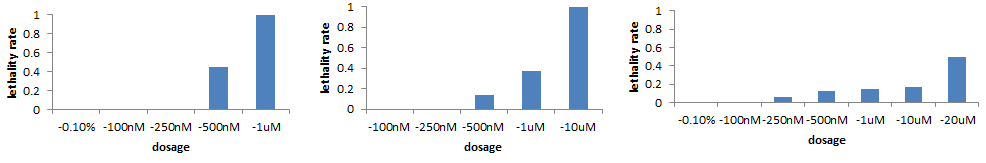
\includegraphics[scale=0.7]{figure/lethalityISV.png}
  \end{center}
  \caption[Effect of varying dosage on ISV]{Lethality rate for three chemicals on ISV. There is an increase in lethality rate with increase in dosage. 0.1\% represents the untreated (control) zebrafish image.}
  \label{lethalISV}
\end{figure}

\begin{figure}[H]\centering
  \begin{center}
    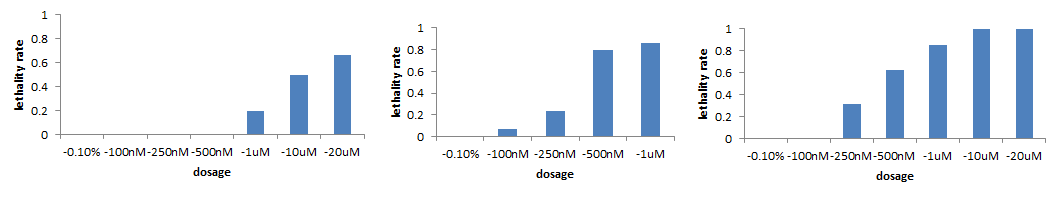
\includegraphics[scale=0.7]{figure/lethalityCVP.png}
  \end{center}
  \caption[Effect of varying dosage on CVP]{Lethality rate for three chemicals on CVP. There is an increase in lethality rate with increase in dosage. 0.1\% represents the untreated (control) zebrafish image.}
  \label{lethalcvp}
\end{figure}
\end{landscape}

Based on lethality rate, we deduced out of 38 screened chemicals, our ISV model identified 28 chemicals that severely ($\geq$ 10\% of embryos are impacted for each dosage within each chemical) impacted ISV growth. Out of 28 chemicals impacting ISV growth, 22 of them showed increasing lethality rate with increasing dosage. Remaining 6 chemicals did not show an increment in lethality rate with increasing dosage, but the effects are more sever at high dosages. Figure \ref{lethalISV} shows lethality rate for three chemicals with increasing dosage. Its worth pointing out that in some cases our model identified untreated zebrafish as unhealthy. Reasons for the miss-classification is due to the imaging artifact. There are 20 images out of 2039, in which zebrafish turned on its back during imaging. We have isolated those images while calculating lethality rate. We can calculate safe dosage as maximum dosage within each chemical with 0 lethality rate.

On similar line as above, we computed lethality rate for CVP analysis. 30 chemicals out of 38 severely ($\geq$ 10\% of embryos are impacted for each dosage within each chemical) impacted development in CVP region. Out of 30 chemicals impacting CVP, 15 showed increasing impacts on CVP with increasing dosage (in terms of lethality rate). Figure \ref{lethalcvp} shows lethality rate for three chemicals with increasing dosage.



\begin{figure}[H]\centering
  \begin{center}
    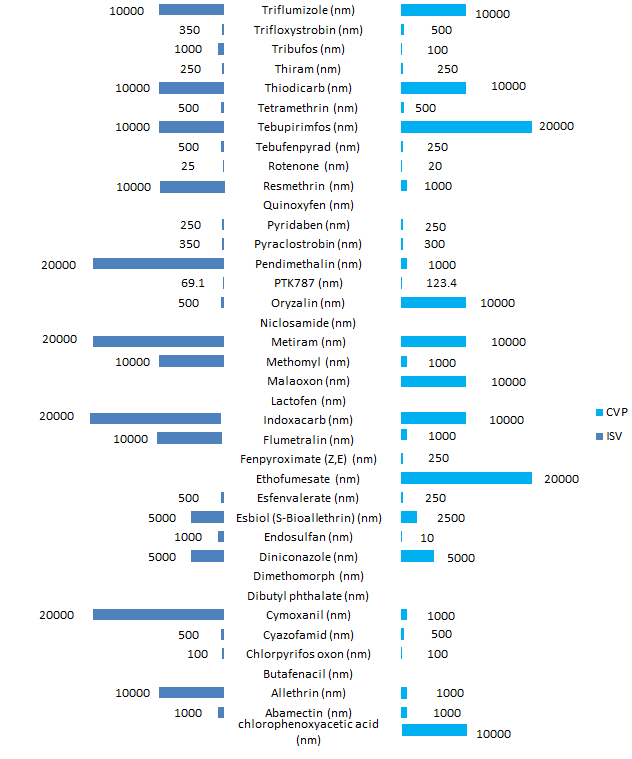
\includegraphics[scale=0.8]{figure/chemicalProfile.png}
  \end{center}
  \caption[Safe Dosage for ISV and CVP]{Figure tells us chemicals, which impact ISV only, CVP only, both ISV and CVP. Safe dosage for each chemical for ISV and CVP region is also illustrated in this plot. Each dosage is given in nanometer (nm). Chemical with the blank value, shows there is no impact due to toxicity for tested dosages.}
  \label{lethalcvpisv}
\end{figure}

A representation is illustrated to show what is the safe dosage for chemical based on ISV and CVP based screening ( fig.\ref{lethalcvpisv}) . This illustration also tells us which chemicals impacted ISV only, CVP only or both ISV and CVP. Moreover it tells us the safe dosage for various chemicals used to treat zebrafish embryo. For 15 chemicals, we found exactly same safe dosage for both ISV and CVP. In 15, of them difference is one step of dosage. By, one step of dosage we mean, lets say dosages tested are 10nm, 100nm, 250nm for a chemical. ISV and CVP shows 100nm and 250nm as safe dosage respectively. Hence we say dosage difference is one step between ISV and CVP. 4 chemicals had a difference of two steps for safe dosages for ISV and CVP. In remaining 4 the difference is more than two steps.

\section{Vasculature Time - Series Analysis}
The computational framework presented in section \ref{sec:timelapse} is applied to quantify vascular changes in both toxin treated and untreated zebrafish embryos. A uniform B-splines control grid with spacing $[20, 20]$, and 3 grid refinement levels are used. Totally, 7 embryos (5 untreated and 2 treated) are analyzed. Vascular growth is computed using method described in section \ref{sec:timelapse}. Figure \ref{toxicityAvgAs} shows the dynamics of blood vessel growth in terms of average pixel change for untreated and arsenic treated embryos. As seen in the figure, although the overall rate of growth is constant for both treated and untreated embryos, the growth rate for untreated embryos is approximately 5 times higher.  

\begin{figure}[!p]
  \begin{center}
    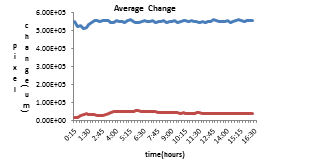
\includegraphics[scale=1]{figure/AvgAs.png}
  \end{center}
  \caption[Average comparison between healthy and treated]{Blue curve shows average change in number of pixels over all the unexposed embryos whereas red curve shows average pixel change for arsenic treated embryo.}
  \label{toxicityAvgAs}
\end{figure}

Figure \ref{toxicityAllAs} shows the dynamics of blood vessel growth in terms of average pixel change for each of the seven embryos analyzed. Pixel change measured in untreated fish is represented by uexposed1 - uexposed5 and exposed1 - exposed2 shows pixel change measured for arsenic exposed embryos.
\begin{figure}[!p]
  \begin{center}
    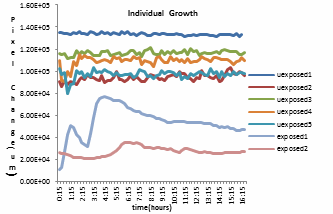
\includegraphics[scale=1]{figure/AllAs.png}
  \end{center}
  \caption[Individual comparison between healthy and treated]{uexposed1 - uexposed5 represents change in number of pixels for unexposed embryos growth, whereas exposed1 and exposed2 represents change in number of pixels for arsenic treated embryos.}
  \label{toxicityAllAs}
\end{figure}

\chapter{Conclusions and Perspectives}\label{chap:conclusion}

As the application of zebrafish in research is becoming more sought after, manual analysis of images has become a bottleneck. This thesis has described a complete framework for the segmentation, quantification, analysis and classification of zebrafish images for ISV and CVP. We also presented methods for ISV and CVP quantification for applications not limited to toxicology analysis. Our results show that ISV and CVP analysis can be used to capture the effect of vascular disruptors. 

Roughly 80,000 industrial chemicals are registered on the US market, and very few of them have been screened for disrupting properties. Thus, development of high throughput screening models that can recognize impacts of toxicity can prove to be very vital. The work presented in this thesis, paves the way for all existing research which has been restricted by analyzing huge amount of data. In conclusion, this work will directly impact the transition from qualitative observation to quantitative measurement of zebrafish by not only providing effective segmentation, but also capturing effective dynamics.


\section{Discussion and Limitations}

Zebrafish being a versatile model, is used in analysis of many biological processes, toxic analysis, and drug screening. Despite the potential of the zebrafish as a model, the actual number of analysis reported is small, involving limited numbers of compounds, with analysis performed manually. Many of the studies reported on zebrafish, focuses on ISV, and yet the research to segment and extract the features from ISV has not taken a lift. The ISVs are particularly interesting because their pattern appears to be established primarily, unlike other vessels such as those of the yolk, brain or retina. Thus, ISVs can give us an initial pathway guidance for capturing dynamics related to growth or environmental cues. 

The key bottleneck restricting these analysis is quantification of the high-throughput experiments, because there are few image analysis methods capable of capturing the complexity ISV. The huge amount of data generated for analysis makes manual analysis a time-inhibiting and error prone process subject to inter-observer variations. Computer-based image processing methods are the only viable way to analyze and quantify the data. Current methods analyze images based on pixel information and thresholding. These methods perform well on clearly resolved objects against a uniform background but often struggle with images that possess information with variable sizes, noise, and heterogeneity across images. This is exemplified in many studies where zebrafish vascular became quantifiable only after manual identification or manual analysis. 

In this work, we focus on developing an integrated image processing methodology to analyze zebrafish embryos post chemical treatment. The pipeline consists of Segmentation of the zebrafish embryo, Region Detection, ISV Extraction, and ISV refinement. We quantify extracted ISV to capture the effect of chemical treatment. A critical issue with the quantitative analysis of zebrafish is that it should be invariant to orientation of zebrafish, and it is highly desirable to have a description that is invariant to noise, intensity
and scales. Our algorithm takes care of this critical issue.

ISV segmentation method perform reasonably well for noisy and blur data (fig. \ref{segISVLim}A and \ref{segISVLim}B). Our method does not perform well for very noisy and blurred ISV (fig. \ref{segISVLim}A and \ref{segISVLim}B near the tail region). Also, ISVs shows immense variation in size. They grow small and thin near the end points, as opposed to center as depicted in figure \ref{segISVLim}D and thin again near head region. Our method is limited by very thin and faded vessels. In figure \ref{segISVLim}D faded vessel does not show in our segmentation. Lastly for figure \ref{segISVLim}C, since ISV curled around zebrafish head, we missed many vessels which does not respond within direction parameters of our method.

\begin{figure}[H] 
 \centering
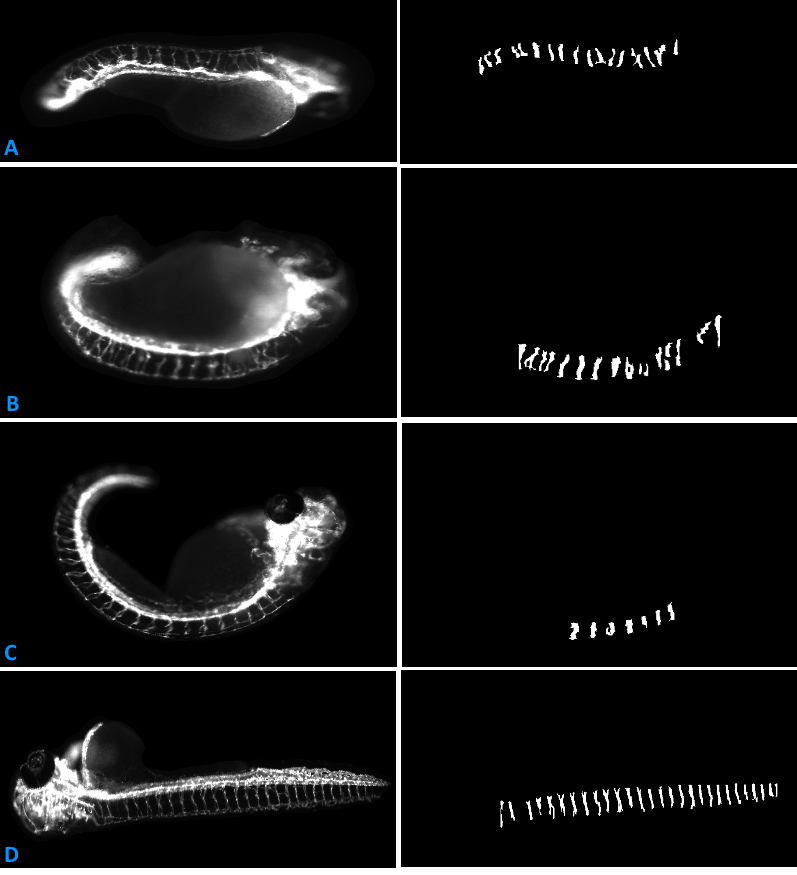
\includegraphics[scale=0.45]{figure/segISVLim.png}
  \caption[Images with the blurred and noisy ISV]{(A), (B) The vessels are more noisy and blurry (C) We lost ISV, due to direction limitation opposed to in tail region. (D) ISVs occur in various sizes, with weak boundary response. Vessels that does not produce a strong response during eigenanlysis also gets excluded during segmentation. Overall, Our algorithm did segmentation of most of ISV. Parameter selection for ISV response and merging causes some loss in data.}
 \label{segISVLim}
\end{figure}



Choice of our parameter effects ISV merging. ISVs remain disjoint is they do not lie within parameter range. In order to negate the effect of direction restriction, we also get response from ISV image in all direction as the probable ISV pixels. Morphological closing operation is applied on direction based ISV and later merged with direction free ISV response. This helps us merge vessels, but if there is no response from direction free ISV, they remain unlinked.

The developed segmentation presents several advantages. Firstly, the parameters are established directly from images so that user interaction is minimal. Secondly, it is not iterative and it can be performed rapidly. Thirdly, this method performs well for images with varied intensity profile and varied texture, orientation and size. Hence, this method possesses the capacity to capture highly dynamic vessels, regardless of phenotype types that exhibit a wide range of morphologies.

We have presented method for segmentation and analysis for CVP. CVP segmentation is based on prior knowledge about change in curvature around tail region. If, our algorithm is not able to find point with the steepest change in curvature, we assume the point where tail starts is the mid point of the curve tracing tail + yolk region. High toxicity impacts the structure of zebrahish, hence perturbing tail region. In those, cases we resort to mid point of curve, which does the good job capturing CVP structure properties. But, it captures more then CVP region (fig. \ref{segISVLim}A, \ref{segISVLim}B, \ref{segISVLim}C). 


\begin{figure}[H] 
 \centering
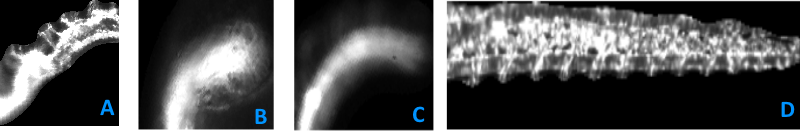
\includegraphics[scale=0.6]{figure/segCVPLim.png}
  \caption[Images with the blurred and noisy CVP]{(A), (B), (C) The tail vessel is structurally damaged due to high dosage. We do get a good estimate of CVP region, but not exact. (D) We are able to segment CVP region well.}
 \label{segCVPLim}
\end{figure}

\section{Future Work}

\textbf{Segmentation}
\newline
In terms of related work, there is a definitely a place for improvement of segmentation of ISV and CVP. Some zebrafish curve around its head under the influence of chemicals. Peng et al. \cite{peng2008} proposed method to straighten curved worm based on formulating the backbone of a worm as a parametric cubic spline defined by a series of control points. This method, can be applied to backbone of zebrafish. This method will improve both the ISV and CVP segmentation.
\textbf{Features}
\newline
Improvement in segmentation, will concurrently improve extracted features. For CVP analysis fusion of morphological properties, with shape properties may improve the classification accuracy. It will be interesting to be able to fuse model for both ISV and CVP to study the toxicology effects and determine safe dosages from chemicals. There is also a scope to be able to extend ISV and CVP analysis algorithm for various other dimensions including 2D + t, 3D, 3D + t. 
\textbf{Applications}
\newline
We have tested our algorithms for application in toxicology. It can be easily extended for drug screening, gene expression modification, or disease modeling. 
% more screen, more applications.

% 

%\bibliographystyle{abbrv}
\bibliographystyle{acm}
\bibliography{bibliography}
%\bibliography{main,BIB/vcl14}
\end{document}
